\bookpart{图}{Graphs}
\label{part:graphs}
\label{part:discrete-mathematics-and-graph-theory}

\BookPartGuide{%
本部分研究连接结构及其上的查询与计算。信号的读数总有规则的位置索引，许多数据却没有
这种索引：样本之间只有“谁与谁接近”，变量之间只有局部依赖，任务之间只有先后关系。
把个体记为顶点、把直接关系记为边，就得到图。图有意只记录最少的信息——哪些个体直接
相关；边长、容量、相似度、方向和局部函数都要另外补上。

本部分分为五章。第~\ref{chap:graph-objects}章确定图、作用域和矩阵表示，
第~\ref{chap:graph-paths}章定义路径、连通与条件分离，这两章固定要保存的数据和查询的
准确含义。第~\ref{chap:graph-traversal}章用遍历、排序、标记、生成森林、分块、树分解
和团树组织计算，第~\ref{chap:graph-optimization}章在路径、容量、树、匹配与划分约束下
作选择，第~\ref{chap:graph-functions}章变换顶点函数并汇总局部配置。

连接限制了路线和组合选择，却不决定边旁数字是长度、容量还是相似度，也不替局部规则
保存真值表。把函数定义在图的顶点上时，顶点值是待处理的信号，连接关系规定传播和比较
发生在哪些位置；结构可用、目标最优与数值查询正确是需要分别建立的三件事。}

\chapter{图的对象与表示}
\label{chap:graph-objects}

四个二值变量$z_i\in\{0,1\}$，$i\in V=\{1,2,3,4\}$，要同时满足三条局部规则：
$z_1,z_2$恰有一个取$1$；$z_3=1$时必须有$z_1=1$；
$z_4=1$时，$z_2,z_3$至少有一个取$1$。
这三条规则分别只涉及$\{1,2\}$、$\{1,3\}$和$\{2,3,4\}$中的变量，
没有哪一条需要同时读入全部四个变量。
要利用这种局部性，先得把“哪些变量直接出现在同一条规则中”记录下来：
把共同出现的每一对变量连接起来，得到边集
\begin{equation}
  E=\bigl\{\{1,2\},\{1,3\},\{2,3\},\{2,4\},\{3,4\}\bigr\}.
  \label{eq:graph-theory-running-edges}
\end{equation}
这就得到一张图，如图~\ref{fig:graph-theory-running-graph}：左右两个三角形共享顶点$2,3$。

\begin{figure}[htbp]
  \centering
  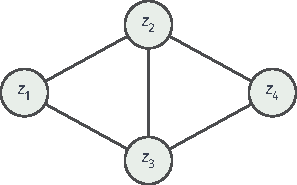
\includegraphics[width=50.281mm]{figures/01-mathematical-preliminaries-upper/07-graphs/tikz/graph-theory-running-graph/figure.pdf}
  \caption{由四变量约束的作用域导出的关系图。边表示两个变量共同出现在至少一个
  约束中；共享顶点集合$\{2,3\}$连接左右两侧。图没有记录约束的具体真值表，
  也没有预先指定边长、容量或相似度。}
  \label{fig:graph-theory-running-graph}
\end{figure}

为什么不直接用向量或矩阵记录这些关系？上一部分的信号总有规则的位置索引，
相邻项就是相邻时刻；矩阵则预设“行对象与列对象两两配对”。
这里的关系是稀疏且不规则的：一个变量可能只与两个同现，另一个却与五个相连，
关系也未必成对出现。用完整矩阵记录，会为大量并不存在的关系预留位置，
更看不出“沿关系能否从一处走到另一处”。因此需要一种只保留
“哪些个体直接相关”的对象，这就是图。

但图有意只记录最少的信息。它只记录哪些个体直接相关，
不记录相关有多强、是什么性质；边表示两个变量共同出现，
却没有保存规则的真值表——三条两两连接并不会把三元规则变成三个等价的二元约束。
边长、容量、相似度、方向和局部函数都要另外补上。
正因为不预设关系的含义，同一种图结构才能同时承担不同任务：
在样本之间表示相似，在变量之间表示统计依赖，在任务之间表示先后次序。

同一条边上附的数字，在不同任务里读法完全不同。
本章先回答“一条边到底保存了什么”：先确定顶点、边、方向与数值属性，
再区分二元关系与高阶关系，然后给出便于计算机使用的矩阵表示，
并顺带建立沿边差分、拉普拉斯与能量这套后两章反复调用的公共算子，
最后说明顶点换名时哪些信息应当保持不变。
固定共享变量$\{2,3\}$以后，左右两侧的局部计算可以分别进行，
这张贯穿图会在本章和后续各章反复出现。

\section{二元关系的图表示}
\label{sec:graph-theory-binary-relations}

本节先确定最基本的图：哪些点、哪些点之间有连接、连接是否带方向，
以及连接上附的数值表示什么。这些属性可以组合——
有向与无向描述方向，加权与无权描述是否附带数值，
并不是几个互斥的图类别。

\subsection{顶点、边与方向}

把每个变量记为一个顶点，把共同出现在一条规则中的一对变量连成边，
边记录的就是直接关系；经过其他变量才能建立的联系暂时不计入。

\paragraph{无向图}
\term{无向图}（undirected graph）写作$\mathcal G=(V,E)$，其中$V$是有限顶点集合，
$E$是由不同顶点的无序对组成的边集合。本章默认不考虑自环（一个顶点连到自身），
也不考虑同一对顶点之间的平行边；若要允许它们，就得另外保存边的身份或重数，
不能继续把边集当成普通无序对集合。若$\{i,j\}\in E$，称$i,j$相邻，二者互为邻居。

\paragraph{邻域}
顶点$i$的\term{邻域}（neighborhood）是它的全部邻居：
\[
  N(i)=\{j\in V:\{i,j\}\in E\}.
\]
在贯穿图中可以逐条读出$N(2)=\{1,3,4\}$、$N(1)=\{2,3\}$。
“枚举$i$的邻居”输出的正是这样一份点的列表，它是后面遍历与邻接访问共用的接口。

\paragraph{顶点的度}
邻域的大小称为顶点$i$的（无权）\term{度}（degree）：
\[
  d_i=|N(i)|.
\]
贯穿图中$d_2=3$、$d_1=2$。度只统计直接邻居的个数，
不统计沿边经过若干步才能到达的顶点；后者要到下一章讨论路径时才计算。
带权时另有“\term{加权度}”，那是把邻边权重累加起来，放在本章拉普拉斯一节定义，
不要与这里的邻居数混为一谈。

\paragraph{有向图与弧}
当关系具有方向——“$i$依赖$j$”与“$j$依赖$i$”是两条相反的信息，
任务依赖、概率生成和网页链接都天然不对称——无序对就不够用了。
\term{有向图}（directed graph）写作$\mathcal G=(V,A)$，
其中$A\subseteq V\times V$是有序对（弧）的集合，仍排除$(i,i)$。
弧$(i,j)$记作$i\to j$，表示允许从$i$一步到$j$；它并不自动包含反向弧$j\to i$。
后续矩阵编码统一采用“行是起点、列是终点”的约定。

\paragraph{入邻域与出邻域}
对顶点$j$，指向它的顶点组成入邻域，由它指出去的顶点组成出邻域：
\[
  N^-(j)=\{i:i\to j\},\qquad N^+(j)=\{i:j\to i\}.
\]
二者的大小分别称为\term{入度}（in-degree）与\term{出度}（out-degree）。
它们沿相反方向读取同一条弧，所以报告“邻居”时必须说明是哪一种。
有向图中常把入邻居称为父节点、出邻居称为子节点，
但这只是方向上的称谓；箭头本身不提供因果解释，
本章只使用连接与方向，其概率与生成机制含义留待相应卷册。

\subsection{边的数值与结构}

结构边只说明两点相邻。同一条边上还可以附一个数值，
这个数值在不同任务里代表完全不同的量，算法入口必须先声明它的语义和取值条件。

\paragraph{边长}
把数值解释为长度或成本$\ell_{i,j}$时，它将在沿路线行走时逐条相加，
累计成本越小越有利。这个数不必等于画图时线段的几何长度；
零长度也可能表示一条可以免费通行的结构边。

\paragraph{边容量}
把数值解释为容量$c_{i,j}$时，它限制允许通过这条通道的流量上界。
容量越大，限制越宽松；零容量表示该通道不能输送正流量。
容量不应当作路径成本直接相加，它回答的是“最多能过多少”，不是“经过要付多少”。

\paragraph{相似度权重}
把数值解释为两点的相似程度$w_{i,j}$时，在后面的平滑与划分中，
大权重通常更强地惩罚两端取值的差异。无向权重满足$w_{i,j}=w_{j,i}$，
有向权重则不必对称。

\paragraph{零权边}
由此可见，零值的含义由当前任务决定：免费道路、零容量通道和零相似度是三回事。
无论哪种，零数值都不自动删除结构边。“能否走到”查的是边集，与权重是否为零无关；
线性加权汇总查的才是作用权重。必要时两者要分别保存。

\paragraph{\term{正权支撑}图}
对有限无向非负权图，把真正起作用的边收集起来：
\[
  E_+=\bigl\{\{i,j\}\in E:w_{i,j}>0\bigr\},
\]
称$(V,E_+)$为正权支撑图。后面的拉普拉斯、谱与扩散只受$E_+$中的权重影响，
因为零权边在差分与平均中贡献为零；而长度问题是否允许使用零权边，
仍按该问题自己的规则判断，不能一概而论。

\subsection{限制顶点集与诱导子图}

只研究一部分对象时，不能悄悄改掉它们之间的关系。
给定顶点子集$U\subseteq V$，保留$U$中的顶点，并保留原图中
两端都属于$U$的全部边（有向图则保留两端都在$U$中的全部弧），
得到的图称为$U$上的\term{诱导子图}（induced subgraph），记作$\mathcal G[U]$。

在贯穿图中取$U=\{1,2,3\}$，诱导子图必须保留$\{1,2\},\{1,3\},\{2,3\}$三条边；
若只留下$1-2-3$这两条边，虽然仍是一个子图，却漏掉了边$\{1,3\}$，
因而不是该顶点集上的诱导子图。诱导子图这一操作后面会反复出现：
取祖先图、删除分隔集后的余图、分块时的局部块，本质上都是在某个顶点集上取诱导子图。

\section{高阶关系的因子表示}
\label{sec:graph-theory-higher-order-scopes}

二元关系只能说“哪两个变量同现”。但“$z_4=1$时，$z_2,z_3$至少有一个取$1$”
是一条同时约束三个变量的规则。把它改画成$2$—$3$、$3$—$4$、$2$—$4$三条边，
虽然保留了哪些变量同现，却丢掉了“这三个变量进入同一条规则”的信息。
本节区分“哪些变量共同出现”与“这些变量的哪些取值被允许”，
并为这种高阶规则保留身份。

\subsection{局部函数与作用域}

\paragraph{局部配置与局部函数}
先固定$z_2,z_3,z_4$各自的取值集合（这里都是$\{0,1\}$），
它们的一次联合取值$(z_2,z_3,z_4)$称为一个局部配置。
上述规则可以写成一个$0/1$指示函数
\[
  \phi_{2,3,4}(z_2,z_3,z_4)=
  \begin{cases}
    0,&(z_2,z_3,z_4)=(0,0,1),\\
    1,&\text{其他二值输入}.
  \end{cases}
\]
它读入三个变量的一次赋值，输出该赋值是否满足规则。
这样定义在少数几个变量上、给出成本、权重或可行性的函数，称为局部函数或因子（factor）。

\paragraph{作用域}
一个局部函数需要读取哪些变量，由这些变量的下标集合记录，称为它的作用域（scope）。
这里$\phi_{2,3,4}$的作用域是$\{2,3,4\}$。作用域保存的是输入位置，不保存函数真值表；
同一个作用域上完全可以附不同的函数。因此“知道作用域”与“知道规则内容”是两回事，
记录同现关系并不等于给出了函数的分解。

\subsection{作用域的三种表示}

\paragraph{超边与超图}
要保留“若干变量属于同一个作用域”，最直接的做法是允许一条边包含多个顶点：
每条超边是一个顶点子集，不限于两个顶点，由此得到\term{超图}（hypergraph）。
超边$\{2,3,4\}$在此记录三元作用域；它仍然不保存局部函数的具体取值。

\paragraph{因子图与二部图}
另一种做法把变量和局部函数分成两组节点，只在变量属于某函数作用域时连边。
两组节点内部都没有边的图称为\term{二部图}（bipartite graph）；
按这种方式得到的因子图（factor graph）通常用方形节点表示因子、圆形节点表示变量，
既保留了因子的身份，又标明了每个因子读哪些变量。完整求值仍需另外保存该因子的函数表。

\paragraph{原始关系图}
若不保留因子节点，只把每个作用域内的变量两两相连，
就得到\term{原始关系图}（primal graph），简称原始图。
章首的贯穿图正是按这条规则由三条局部条件得到的：三元作用域$\{2,3,4\}$
贡献了$\{2,3\},\{2,4\},\{3,4\}$三条边。

\paragraph{成对投影的信息损失}
关键问题是：仅靠原始图上的两两关系，能不能恢复原来的高阶约束？一般不能。
考虑三元二值约束“恰有偶数个变量等于$1$”，它允许
$(000,011,101,110)$四种配置。把它投影到每一对变量上，
每一对的四种取值$(00,01,10,11)$都会在某个允许配置中出现，
于是只保留这三个成对允许关系，将不再排除任何配置，连$(001)$也被错误地放行了。

\begin{figure}[htbp]
  \centering
  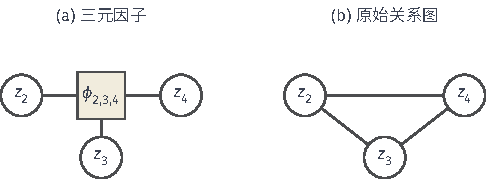
\includegraphics[width=82.282mm]{figures/01-mathematical-preliminaries-upper/07-graphs/tikz/graph-theory-factor-scope/figure.pdf}
  \caption{三元因子与原始关系图。左侧方框是同一个依赖$z_2,z_3,z_4$的函数，
  连线表示作用域归属；右侧只保留变量共同出现的两两关系。右侧三条边不是把三元
  函数分解成三个二元函数的等价变换，也不能恢复原函数的数值。}
  \label{fig:graph-theory-factor-scope}
\end{figure}

如图~\ref{fig:graph-theory-factor-scope}所示，一个三元因子和三个二元因子
可以产生同一个三角形原始图，但前者能表达的约束未必能写成后者同时成立的形式。
因此后续的树分解与变量消元都必须保留完整作用域，不能把原始图当作原约束表。

\section{图的矩阵表示}
\label{sec:graph-theory-matrix-representations}

对象确定之后，还要选一种让计算机能高效使用的表示。
同一种连接结构要支撑性质不同的高频访问：遍历要取出某个顶点的全部邻居，
数值传播要把邻居的值按权重加起来，计算边差则要逐条取出一条边的两端。
本节先比较几种存储结构，再由邻接矩阵和关联矩阵建立邻居汇总与边差，
最后把边差汇总成贯穿全书的拉普拉斯算子及其归一化形式。

\subsection{邻接访问与存储}

\paragraph{邻接表}
遍历要反复枚举一个顶点的全部邻居。\term{邻接表}为每个顶点保存它的邻居及所需边属性。
记$n=|V|$、无向边数$m=|E|$（有向图记弧数$a=|A|$），总存储为$O(n+m)$；
无向边在两个端点各存一次，反向弧表的存储也要计入。

\paragraph{边表}
当算法需要逐条处理边（排序边、扫描边、维护残量配对）时，
\term{边表}直接保存每条边的两个端点、身份与属性。邻接表与边表可以同时使用，
多出的$O(m)$个记录应计入存储代价。

\paragraph{稠密矩阵与稀疏矩阵}
稠密矩阵为每一对顶点都预留位置，占$O(n^2)$存储；稀疏矩阵只保存实际非零条目。
分析算法代价时必须声明采用哪种表示：邻接表上沿邻居的线性遍历，
不能直接套到逐行扫描稠密矩阵上。

\paragraph{邻接矩阵}
固定顶点次序$1,\ldots,n$，\term{邻接矩阵}（adjacency matrix）
$\bm A\in\mathbb R^{n\times n}$的条目为
\[
  a_{i,j}=
  \begin{cases}
    w_{i,j},&\{i,j\}\in E\ \text{或}\ (i,j)\in A,\\
    0,&\text{其他情形},
  \end{cases}
\]
无权边取权重$1$。贯穿图对应
\begin{equation}
  \bm A=
  \begin{bmatrix}
    0&1&1&0\\
    1&0&1&1\\
    1&1&0&1\\
    0&1&1&0
  \end{bmatrix}.
  \label{eq:graph-theory-running-adjacency}
\end{equation}

\paragraph{矩阵乘法的方向}
有向情形按“行起点、列终点”约定：
\[
  (\bm A\bm f)_i=\sum_j a_{i,j}f_j
\]
读出的是顶点$i$的出邻居值之和；$\bm A^\top\bm f$则把每个起点的值沿出弧发送到终点。
图~\ref{fig:vol1-add-graph-adjacency-orientation}用只有两条弧$1\to2,1\to3$、
$\bm f=(1,2,3)^\top$的小图分别算出$\bm A\bm f=(5,0,0)^\top$（顶点$1$读取$2+3$）
和$\bm A^\top\bm f=(0,1,1)^\top$（把$f_1=1$送到两个终点）。
无向图中$\bm A$对称，两种读法才重合。
\begin{figure}[!htb]
  \centering
  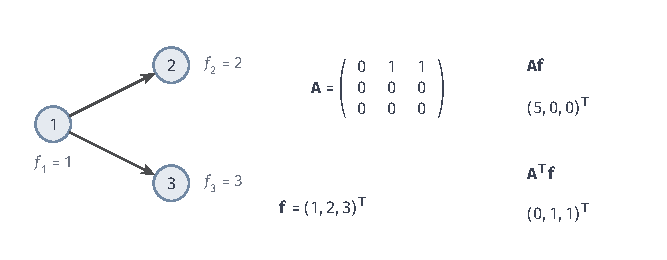
\includegraphics[width=112mm]{figures/01-mathematical-preliminaries-upper/00-shared/tikz/graphs-and-signals-comprehension-additions/graph-adjacency-orientation.pdf}
  \caption{只有两条单位权弧$1\to2$和$1\to3$的有向图，顶点值为$\bm f=(1,2,3)^\top$。
  邻接矩阵按“行起点、列终点”存储：$\bm A\bm f$在顶点$1$处读取$2+3=5$；
  $\bm A^\top\bm f$则将$f_1=1$沿两条弧发送，顶点$2,3$各收到$1$。
  矩阵转置改变汇总方向，未改变图中弧的定义。}
  \label{fig:vol1-add-graph-adjacency-orientation}
\end{figure}
在贯穿图上取$\bm f=(1,2,3,4)^\top$，可复算$\bm A\bm f=(5,8,7,5)^\top$。
这是顶点值的线性汇总，不等于在全部变量配置上求和，后者还需要明确局部因子。

\paragraph{结构掩码}
允许零权边时，数值$0$无法区分“无边”与“零权边”。
为此另存一个结构掩码$\bm M\in\{0,1\}^{n\times n}$：存在结构边或弧时$m_{i,j}=1$，否则为$0$。
后续算法要说明自己读的是数值矩阵还是结构掩码；例如两顶点空图与两顶点零权单边图
都可能有$\bm A=\bm 0$，连接关系却不同。

\subsection{关联矩阵与边差}

\paragraph{关联矩阵}
要计算每条边两端的差，给每条无向边任选一个临时方向，构造\term{关联矩阵}
（incidence matrix）$\bm B\in\mathbb R^{n\times m}$：
边$e$从$i$指向$j$时，对应列在$i$处取$1$、在$j$处取$-1$，其余为零。
于是
\[
  (\bm B^\top\bm f)_e=f_i-f_j
\]
正好是该边两端的差。临时方向只用于统一记录这个差值。

\paragraph{边差的加权汇总}
令$\bm W_E=\operatorname{diag}(w_e:e\in E)$为边权对角矩阵，则
$\bm B\bm W_E\bm B^\top$分三步完成“取边差—按边权缩放—汇总回顶点”。
若反转某些边的临时方向，相当于右乘一个对角元为$\pm1$的符号矩阵$\bm R$
（反向的边取$-1$，其余取$1$）：$\bm B'=\bm B\bm R$。
由于$\bm R\bm W_E\bm R=\bm W_E$，所得无向加权算子并不随临时方向改变。
这一便利只属于无向边的临时定向，不能用来消除真正有向图中的方向。

\subsection{组合拉普拉斯与沿边变化}

下面把边差汇总成一个算子。这套算子是第~\ref{chap:graph-optimization}章图划分与第~\ref{chap:graph-functions}章谱方法、扩散共用的基础，
因此在此一次性建立；如何用它做离散优化、如何按谱滤波，则分别留给那两章。

\paragraph{加权度}
固定有限无向、权重非负的图。顶点$i$的加权度及其对角矩阵为
\[
  d_i^{(w)}=\sum_j w_{i,j},\qquad
  \bm D^{(w)}=\operatorname{diag}(d_1^{(w)},\ldots,d_n^{(w)}).
\]
无权度$d_i$数的是邻居个数，加权度$d_i^{(w)}$累计的是相邻边的作用强度；
只有每条结构边权均为$1$时二者才相同。

\paragraph{组合拉普拉斯}
\term{组合图拉普拉斯}（combinatorial graph Laplacian）定义为
\begin{equation}
  \bm L=\bm D^{(w)}-\bm W=\bm B\bm W_E\bm B^\top,
  \label{eq:graph-theory-combinatorial-laplacian}
\end{equation}
其逐点作用为
\[
  (\bm L\bm f)_i=\sum_j w_{i,j}(f_i-f_j).
\]
它把本点值与各邻居值之差按权重汇总；相邻值已经相等的边不再贡献。
每条边给两端对角元各加$w_e$、给两个交叉位置各加$-w_e$，合计正是$\bm D^{(w)}-\bm W$。
常数向量满足$\bm L\bm 1=\bm 0$，因为常数在每条边上都没有差异。

\paragraph{沿边变化能量}
拉普拉斯对应的二次型把全部边差平方按权重累加起来：
\begin{equation}
  \bm f^\top\bm L\bm f
  =\sum_{\{i,j\}\in E}w_{i,j}(f_i-f_j)^2
  =\frac12\sum_{i,j}w_{i,j}(f_i-f_j)^2.
  \label{eq:graph-theory-dirichlet-energy}
\end{equation}
两种写法只是计数方式不同：按无向边$\{i,j\}$求和每条边计一次，无需系数；
按有序对$(i,j)$求和每条边计两次，因此乘$1/2$。
因为权重非负、每项是平方，这个量恒非负，所以$\bm L$对称半正定。
若边权允许为负，非负性便不再成立；真正的有向图也另有不同的拉普拉斯，
不能直接套用这里的对称谱结论。

\paragraph{零能量的逐边条件}
二次型为零，当且仅当每一个平方项都为零，即每条正权边的两端值相等：
\[
  \bm L\bm f=\bm 0
  \quad\Longleftrightarrow\quad
  f_i=f_j\ \text{对所有}\ \{i,j\}\in E_+.
\]
零权结构边不强制两端相等。例如一条结构边仍在但权为$0$，
它两端取不同值也不会使能量变大。至于“沿正权边把相等关系传遍一个连通分量、
从而零空间由各分量常数组成”这一完整刻画，要用到下一章才正式建立的路径与连通分量，
因此放在第~\ref{chap:graph-functions}章谱方法入口完成；这里只确定逐边条件本身。

\subsection{归一化算子与度量}

组合拉普拉斯直接比较顶点值。但同样的端点差，在连接很多的顶点上会被累计更多次；
有时希望把连接总量也计入顶点幅度的衡量。这就需要归一化。
本节的共同前提是无向、非负权重；零度顶点要单独约定。
本节起$d_i$一律是加权度$d_i^{(w)}$的简写，不再表示邻居数。

\subsubsection{对称归一化拉普拉斯}

\paragraph{度加权内积与坐标缩放}
在正度顶点构成的子空间上，用度给长度加权：
$\langle\bm g,\bm h\rangle_{\bm D}=\bm g^\top\bm D^{(w)}\bm h$。
为了继续使用普通欧氏内积下的正交谱，作坐标变换
\begin{equation}
  \bm f=(\bm D^{(w)})^{1/2}\bm g,\qquad
  \bm f^\top\bm f=\bm g^\top\bm D^{(w)}\bm g,
  \label{eq:graph-theory-degree-coordinates}
\end{equation}
它把度加权长度换成普通欧氏长度。含零度点时$\bm D^{(w)}$在全空间退化，
不能把该式称为全空间内积，相关结论都限制在正度子空间。

\paragraph{对称归一化拉普拉斯的定义}
把同一代换送入边差能量，得到\term{对称归一化拉普拉斯}
（symmetric normalized graph Laplacian）
\begin{equation}
  \bm L_{\mathrm{sym}}
  =(\bm D^{(w)})^{-1/2}\bm L(\bm D^{(w)})^{-1/2}.
  \label{eq:graph-theory-normalized-laplacian}
\end{equation}
正度部分按公式定义；对$d_i^{(w)}=0$的支撑孤立点，约定逆平方根条目取$0$，
相应行列为零。不能对零直接取倒数，也不应在这个约定下把孤点对角元写成$1$。

\paragraph{归一化后的沿边能量}
展开二次型可得
\[
  \bm f^\top\bm L_{\mathrm{sym}}\bm f
  =\sum_{\{i,j\}\in E_+}w_{i,j}
    \left(\frac{f_i}{\sqrt{d_i}}-\frac{f_j}{\sqrt{d_j}}\right)^2\geq 0.
\]
求和只对正权边$E_+$进行，这些边的两端加权度都为正，故不会除零；
零度点没有正权邻边，单独贡献$0$。这里比较的是度缩放之后的值，与组合拉普拉斯比较原值不同。

\paragraph{归一化谱界}
对任意实数$a,b$有$(a-b)^2\leq 2(a^2+b^2)$。逐条边相加，每条边把
$a_i^2$、$a_j^2$各计入一次，而$\sum_j w_{i,j}=d_i$，于是
\[
  0\leq \bm f^\top\bm L_{\mathrm{sym}}\bm f\leq 2\bm f^\top\bm f.
\]
由Rayleigh商，$\bm L_{\mathrm{sym}}$的特征值全部落在$[0,2]$；
零度孤立点对应的零特征值也在此区间内。这条谱界后面构造按$2$缩放的谱滤波时会直接用到。

\subsubsection{邻域平均与随机游走拉普拉斯}

\paragraph{邻域平均算子}
在正度部分定义逐行归一化的邻域平均矩阵
\[
  \bm P_{\mathrm{rw}}=(\bm D^{(w)})^{-1}\bm W.
\]
它每行权重和为$1$，$(\bm P_{\mathrm{rw}}\bm f)_i=\sum_j(w_{i,j}/d_i)f_j$
是从顶点$i$读取其邻居的加权平均。下标$\mathrm{rw}$提示它与随机游走相关，
也借此与重编号用的置换矩阵$\bm P$区分。零度孤立点约定$(\bm P_{\mathrm{rw}})_{i,i}=1$、
该行其余条目为$0$，使读取在孤点处保持原值。

\paragraph{随机游走拉普拉斯}
本点值减去邻居平均，得到\term{随机游走拉普拉斯}
\[
  \bm L_{\mathrm{rw}}=\bm I-\bm P_{\mathrm{rw}},
\]
在正度部分等于$(\bm D^{(w)})^{-1}\bm L$，孤立点对应零块。
这个名称允许把归一化系数解释为“下一步选择某邻居的概率”，
但完整的随机游走与Markov链还需指定随机序列和转移规则，这里只做有限权重的归一化。

\paragraph{两种归一化算子的关系}
在正度部分，
\[
  \bm L_{\mathrm{rw}}
  =(\bm D^{(w)})^{-1/2}\bm L_{\mathrm{sym}}(\bm D^{(w)})^{1/2},
\]
所以二者相似、共享特征值。$\bm L_{\mathrm{rw}}$一般不在普通欧氏内积下对称，
但由$\bm D^{(w)}\bm L_{\mathrm{rw}}=\bm L=\bm L^\top$可知，
它在度加权内积$\langle\cdot,\cdot\rangle_{\bm D}$下自伴；
有零度点时这一判断要限制到正度子空间。

\paragraph{函数读取与概率质量推送}
若把行随机矩阵进一步解释为转移概率，要区分两种读法：
读取顶点上的函数值用$\bm f\mapsto\bm P_{\mathrm{rw}}\bm f$，
推送一列概率质量则用$\bm p\mapsto\bm P_{\mathrm{rw}}^\top\bm p$。
这与前面邻接矩阵“读取邻居、沿出弧发送”的方向约定一致。
稳态、混合等完整结论由概率卷建立，此处不提前承诺任何收敛性质。

\begin{table}[htbp]
  \centering\small
  \begin{tabularx}{\linewidth}{@{}lX@{}}
    \toprule
    算子 & 内积与每个连通分量的零模\\
    \midrule
    $\bm L$ & 欧氏内积；分量内顶点值为常量，零模为分量指示向量\\
    $\bm L_{\mathrm{sym}}$ & 欧氏内积，信号坐标按度缩放；
      零模为分量上的$\sqrt{d_i^{(w)}}$向量\\
    $\bm L_{\mathrm{rw}}$ & 度加权内积下自伴；分量内顶点值为常量\\
    \bottomrule
  \end{tabularx}
  \caption{同一非负权图的三种拉普拉斯几何。表中假设全部顶点为正度，
  “分量”均指正权支撑图的连通分量；零度点按正文约定另行处理。改变坐标与改变内积是两种不同操作，
  不能把三种算子的特征向量直接互换。}
  \label{tab:graph-theory-laplacian-geometries}
\end{table}

\section{重编号下的结构等价}
\label{sec:graph-theory-graph-isomorphism}

画在纸上的图带有顶点名称，但名称往往是任意的。若把贯穿图的顶点换一套名字，
邻接矩阵的行列会跟着移动，连接本身却没有改变。比较两张图时，
应当允许顶点名称之间存在一个保持边关系的一一对应。本节确定“只是换名”要保留什么，
并指出矩阵谱在这个问题上的能力边界。

\paragraph{图同构}
两图$\mathcal G=(V,E)$、$\mathcal G'=(V',E')$若存在双射$\rho:V\to V'$，使
\[
  \{i,j\}\in E
  \quad\Longleftrightarrow\quad
  \{\rho(i),\rho(j)\}\in E',
\]
就称二者\term{同构}（isomorphic）：忽略顶点名称后，连接结构完全相同。
双向箭头同时排除了丢失原边和引入额外边两种错误。有向图同构还要求保持有序弧，
加权图要保持对应权重，带属性图则要说明哪些属性也必须保持。

\paragraph{置换矩阵与坐标重排}
设置换矩阵$\bm P$满足$(\bm P\bm f)_{\rho(i)}=f_i$，重编号在矩阵上表现为
\begin{equation}
  \bm A'=\bm P\bm A\bm P^\top.
  \label{eq:graph-theory-adjacency-relabel}
\end{equation}
这是置换共轭，只把坐标搬来搬去，不把两个顶点的数值混合；
而一般相似变换允许混合坐标，所以不能把任意换基都解释成图的重编号。
允许零权结构边时还要同时检验结构掩码$\bm M'=\bm P\bm M\bm P^\top$，
因为两顶点空图与两顶点零权单边图可以有相同的数值矩阵$\bm A=\bm 0$。

\paragraph{同谱图与同构的边界}
置换共轭是相似变换，所以同构图必有相同的邻接谱；但反过来不成立。
四叶星图$K_{1,4}$与“一个四环加一个孤立顶点”都具有邻接特征值
$\{2,-2,0,0,0\}$，但前者连通、后者不连通，显然不同构。
因此同谱只是同构的必要条件而非充分条件。这里比较的是邻接谱；
组合拉普拉斯、归一化拉普拉斯各有自己的谱，不能笼统地说“两图频率相同”。
第~\ref{chap:graph-functions}章讨论图上函数的等变性与区分能力时，会回到这里建立的比较标准。

\section{本章小结}

回到章首的四变量规则，可以把一条边上保存的信息逐层分清：
结构边只说明两个变量同现；边旁数字要先声明是长度、容量还是相似度；
作用域记录一个局部函数读哪些变量，函数表才记录这些变量的哪些取值被允许。
图表示、因子表示和矩阵编码是同一对象的不同侧面，
拿到任务时要检查这几类输入是否齐全。

本章还建立了三组需要分清的关系。其一是结构与数值：
能否通行查边集与结构掩码，数值传播查作用权重，零权边仍在但不贡献差分。
其二是读取方向与推送方向：$\bm A\bm f$读出邻居、$\bm A^\top\bm f$沿弧发送，
邻域平均读函数用$\bm P_{\mathrm{rw}}\bm f$、推概率质量用其转置。
其三是同构与同谱：重编号对应置换共轭，同构必同谱，但同谱不足以保证同构。
组合拉普拉斯及其两种归一化，连同各自的内积、能量和零空间约定，
是后面图划分与图滤波共用的算子基础。

下一章在这些对象上定义路径、连通与条件分离，回答“沿连接能到哪里、
给定一部分顶点后两端是否还相连”；本章不提前展开这些查询的检索算法。

\chapter{图中的路径与连接关系}
\label{chap:graph-paths}

第~\ref{chap:graph-objects}章固定了图上要保存的数据：哪些点相邻、边朝哪个方向、边上附的是什么数值。
本章在这些对象上提出查询。贯穿图里顶点$1$和$4$并不相邻，却可以经过$2$或$3$相连；
正是“不能一步到达、但能沿若干条边到达”这一观察，引出了本章的四类问题。

第一类问一步能到谁，答案就是邻域，只查边集和方向。第二类问怎样沿一串边走到目标，
要先规定允许经过什么样的顶点序列，以及沿路线累计什么成本。
第三类问一批顶点是否彼此可达：无向图用连通分量把顶点分成互相可达的块，
有向图还要区分单向可达与双向可达。第四类问得更细——
已知一部分顶点的取值后，另外两组顶点之间是否还存在能传递信息的通路；
这在概率模型里对应条件独立，但它首先是一个图上的判据。

四类查询检查的对象从一条边扩展到一条路线、再扩展到所有路线之间的整体关系，
但这并不意味着计算难度严格递增，实际代价取决于图的表示和具体算法。
本章只建立判定对象与条件：什么样的序列算路径、什么情况下两点算连通、
一条底层路径在给定条件集下何时活跃。怎样用队列、栈真正检索这些关系，
以及怎样把一次条件分离查询变成无向可达查询，是第~\ref{chap:graph-traversal}章的内容。

\section{顶点之间的邻接关系}

邻接查询只回答“能不能走一步”。在贯穿图中，$1,2$相邻而$1,4$不相邻，
$1,4$必须经过中间点才能相连。改成有向图后还要看方向：弧$i\to j$允许一步从$i$到$j$，
不能据此反向通行。

同一条结构边上的数值只是在修饰已声明的关系，查询邻接时不应拿数值当门槛。
若数字是长度$5$，经过它付出成本$5$；若是容量$5$，它限制总通过量；
若是相似度$5$，它通常鼓励两端取值接近。零长度可表示免费通行，
零容量表示不能承载正流量，零相似度表示不贡献加权差分，但三者都不自动删除结构边。
因此“这两个顶点之间能否走一步”应查边集及方向，而不是检查某个数值矩阵的条目是否大于零。

\section{顶点之间的路径关系}

\subsection{行走、路径与环}

把相邻的边首尾相接，就得到顶点的序列。这里要区分三个层层收紧的对象，
因为它们服务的计算不同。

\paragraph{行走}
\term{行走}，也称\term{游走}（walk），是顶点序列$v_0,v_1,\ldots,v_k$，
每对相邻项$v_{r-1},v_r$之间都有边，允许重复经过顶点和边；边数$k$称为行走的长度，
单个顶点算长度为零的行走。贯穿图中$1,2,3,1,2$就是一条行走，
它重复经过了顶点$1,2$。反复传播、沿环不断循环这一类过程，用行走描述最自然。

\paragraph{简单路径}
若序列中的顶点两两不同，就称为简单\term{路径}（path）。
本部分无修饰的“路径”默认指简单路径，对应一条不重复经过对象的具体路线；
单个顶点仍是长度为零的路径。$1,2,4$是贯穿图中的一条路径，
它与允许重复的行走$1,2,3,1,2$形成对照。

\paragraph{闭行走与无向环}
首尾相同（$v_0=v_k$）的行走称为闭行走。在无向简单图中，
若除首尾重合外$v_0,\ldots,v_{k-1}$两两不同且长度$k\geq3$，就得到简单\term{环}（cycle）。
$1,2,3,1$是一个环；沿同一条边走过去再退回来虽然闭合，却不构成环，
因为中间顶点并不满足互异条件。

\paragraph{有向路径与有向环}
有向行走与\term{有向路径}（directed path）的每一步都必须沿弧方向。
\term{有向环}（directed cycle）除首尾重合外顶点互异，且闭行走的每一步都顺着弧。
在排除自环的有向图里，环可以短到两条弧：$i\to j$与$j\to i$合起来就是长度$2$的有向环。

\paragraph{有向无环图}
不含有向环的有向图称为\term{有向无环图}（directed acyclic graph, DAG）。
这里的“无环”只针对有向环，不要求忽略方向后的底层图也无环：
$1\to2$、$1\to3$、$2\to3$构成DAG，但把箭头去掉后是一个三角形。
这一区别在第~\ref{chap:graph-traversal}章拓扑排序时很关键——排序要求的是有向无环，不能替换成“底层图无环”。

\paragraph{邻接矩阵幂与行走计数}
邻接矩阵的幂可以直接检索行走，却不会替我们排除重复顶点。
对无权图，$(\bm A^k)_{i,j}$恰好等于从$i$到$j$长度为$k$的行走数。
$k=0$时$\bm A^0=\bm I$记录留在原地的零步行走；归纳地，按倒数第二个顶点$\ell$分类：
\[
  (\bm A^{k+1})_{i,j}=\sum_\ell(\bm A^k)_{i,\ell}a_{\ell,j},
\]
每条长度$k+1$的行走被计数恰好一次。带权时条目变成
$\sum\prod_r w_{v_{r-1},v_r}$，即每条行走的权重乘积之和，
既不是行走条数，也不是边长之和。把加法、乘法换成布尔运算或最小加法，
可回答可达性或固定步数最低成本，但那已经更换了矩阵运算规则，
其统一依据留到第~\ref{chap:graph-functions}章的半环一节。

\subsection{路径成本与最短距离}

\paragraph{路径成本}
当边的任务是记录长度或代价时记作$\ell_{i,j}$，以免与相似度混淆。
路径$P=(v_0=s,\ldots,v_k=t)$的成本是所经边成本之和
\[
  \ell(P)=\sum_{r=1}^k\ell_{v_{r-1},v_r}.
\]
所有边长都是$1$时，最小成本等于最少边数；一般边长下两者不等价。
例如$s$与$t$之间一条直达边长$5$，而经$u$的两条边各长$1$，两步路径反而更短。

\paragraph{简单路径最小值与行走下确界}
是否允许重复经过顶点，会改变候选集合。有限图的简单路径只有有限条，
所以只要可达，简单路径成本就有最小值；允许行走时候选数可以无限，
此时更自然的是谈成本的下确界。后续距离递推默认针对允许重复的有限行走，
不能不加说明地在两种候选对象之间切换。

\paragraph{负闭行走}
如果能从源$s$走到一个成本为负的闭行走，绕完它之后又能继续通往目标$t$，
那么每多绕一圈成本就再降低一次，反复绕行使目标的行走成本下确界为$-\infty$。
这不是说存在一条“长度为负无穷的路径”，而是任意有限成本都能被更小的成本打破。
有向负闭行走必包含一个负有向环；在无向图里，沿一条负边往返一次就构成负闭行走，
即使这条边不在任何无向简单环上。当不存在这种“从源可达、又能到目标”的负闭行走时，
可从行走中删去非负的闭合段而不增加成本，行走问题才与简单路径问题一致。

\paragraph{距离查询的三种状态}
因此一次距离查询可能有三种结果：目标不可达（距离为$+\infty$）、
存在有限最短距离、以及受相关负闭行走影响而下确界为$-\infty$。
如何识别负环并把它的影响传播到全部后继，是第~\ref{chap:graph-optimization}章Bellman--Ford方法要处理的内容；
仅靠“图中没有无向简单负环”这样的说法不足以排除负闭行走。

\section{顶点集合的连通关系}

本节只建立后面方法需要的连接概念，并用最小例子说明。
网格上的$4/8$邻接等专门规则留到第~\ref{chap:graph-traversal}章连通标记方法的输入处按需介绍。

\paragraph{无向连通与连通分量}
若两点之间存在路径，称它们互相可达；长度为零的路径使每个顶点与自身可达。
把彼此可达的顶点归到一起，得到连通分量：每个分量内部任意两点可达，
不同分量之间没有路径。可达关系的自反、对称、传递性保证这些分量构成顶点集的唯一划分。
只有一个分量的非空无向图称为\term{连通}（connected）图。
“三角形加一个孤立顶点”有两个分量，组内可达、组间无路。
还要注意：删除环上的一条边只破坏该环，不一定破坏连通，
是否断开应检查有没有替代路径，而不是只数少了几条边。

\paragraph{祖先与后代}
有向可达要求存在顺弧的路径，因而通常不对称。本章把通过正长度有向路径到达$j$的
其他顶点称为$j$的祖先，把从$j$沿正长度有向路径能到达的其他顶点称为后代，
二者都不含$j$自身；一弧相连的父点只是祖先中的一个。一般有环图里两个不同顶点
可以互为祖先，DAG里则不可能。

\paragraph{强连通与强连通分量}
若任意有序顶点对$i,j$之间都有从$i$到$j$的有向路径，称图\term{强连通}
（strongly connected）；相互可达的极大顶点集称为强连通分量。
链$1\to2\to3$的三个点分属三个强分量，因为虽然$1$能到$3$，$3$却不能返回$1$，
不能把单向到达的点合进同一个强分量。

\paragraph{弱连通}
忽略弧方向后所得无向图若连通，称原有向图\term{弱连通}（weakly connected）。
上面的链只有一个弱连通分量，但弱连通并不保证两点能双向到达。

\paragraph{树与森林}
连通且无环的无向图称为\term{树}（tree）；由若干互不相连的树组成的图称为森林。
树之所以好用，在于“连通保证有路径、无环保证路径唯一”：
树中任意两点间的简单路径恰好一条。这正是树上消息可以分块、
同一局部贡献不会沿不同路线被重复计入的根源。

对含$n\geq1$个顶点的有限无向简单图，下面三条等价：
图连通且无环；任意两点之间恰有一条简单路径；图连通且恰有$n-1$条边。
其理由是直接的：连通性至少给出一条路径，若有两条不同路径，
从它们首次分开处到再次会合处便形成环，故无环时路径唯一；
反之路径唯一已蕴含连通，若有环则环上相邻顶点间既有该边、
又有沿环另一侧的路径，与唯一性矛盾。在此基础上反复摘除叶顶点即可数出$n-1$条边，
而连通且有$n-1$条边时逐点接入恰好得到一棵树，故图本身无环。
但单看“$n-1$条边”不足以判树：三角形加一个孤立顶点有四个顶点、三条边，却不是树。
从一般连通图中抽取一棵覆盖全部顶点的树，需要明确保留哪些连接、舍弃哪些边，
这是第~\ref{chap:graph-traversal}章生成森林方法的任务。

\section{条件约束下的分离关系}
\label{sec:graph-paths-conditional-separation}

前三类查询只涉及边和路径的存在性。最后一类查询给定一个顶点集合$S$，
问忽略方向后连接两端的路径能否“通过条件检查”。本节先讲无向分隔，
再给出DAG中单条路径的活跃规则与d-分离定义；
怎样不必枚举全部路径而完成一次判定，留到第~\ref{chap:graph-traversal}章。

\paragraph{无向分隔}
对两两不交的顶点集合$A,B,S$，其中$A,B$非空，若从$A$到$B$的每条无向路径都经过$S$，
就称$S$把$A$与$B$\term{分隔}（separate）；等价地，删除$S$及其关联边后，
没有连通分量同时包含$A$和$B$的点。在贯穿图取$A=\{1\},B=\{4\}$：
只删$S=\{2\}$仍可经$1-3-4$通行，并未分隔；删$S=\{2,3\}$才把两端分开。
所以必须阻断所有路径——找到一条被阻断的路径，不足以判定两端已分离。

\paragraph{路径中的碰撞点}
沿箭头的可达描述依赖方向；条件分离检查的则是忽略方向后的一条底层路径上箭头如何排列。
先看三个只有一个内部顶点$c$的路径：链$a\to c\to b$与分叉$a\leftarrow c\to b$上，
箭头不在$c$处相汇；而在碰撞结构$a\to c\leftarrow b$上，两支箭头同时指向$c$，
称$c$为该路径上的碰撞点，其余内部顶点为非碰撞点。一个点是不是碰撞点
取决于它在当前路径上相邻两弧的方向，并不是该顶点的固定类别。

\paragraph{给定条件集后的活跃路径}
碰撞点的判断还要沿出弧向后看。沿用前面的后代定义：给定不含路径端点的集合$S$，
一条底层路径\term{活跃}（active），当且仅当它的每个非碰撞内部顶点都不在$S$中，
且每个碰撞点自身或某个后代属于$S$。
于是在链和分叉上，空条件集允许通过、把中点放入$S$则阻断；
在碰撞结构$a\to c\leftarrow b$上恰好相反，空条件集阻断、给定$c$才打开。
若另有$c\to d$，那么即使只给定后代$d$（$S=\{d\}$），碰撞点也算被打开。
这说明条件分离不能靠简单删除$S$后做一次连通检查，还要查看路径外的后代。

\paragraph{d-分离}
\begin{definition}[d-分离]
  \label{def:graph-theory-d-separation}
  设$\mathcal G$为有限DAG，$A,B,S\subseteq V$两两不交且$A,B$非空，
  $S$不含所考察路径的端点。若连接$A$与$B$的每条底层路径在给定$S$时都不活跃，
  称$A,B$被$S$\term{d-分离}（d-separated），记作
  $A\perp_{\mathcal G}B\mid S$；否则称$A,B$被$S$ d-连接。
\end{definition}

\begin{figure}[htbp]
  \centering
  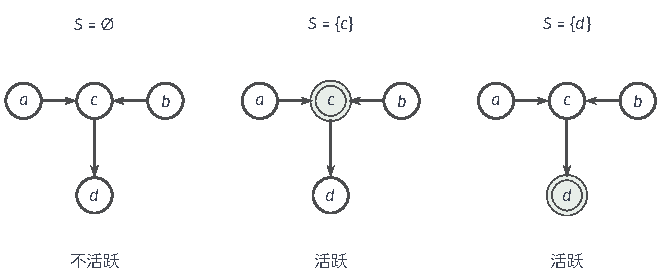
\includegraphics[width=112.0mm]{figures/01-mathematical-preliminaries-upper/07-graphs/tikz/graph-theory-active-paths/figure.pdf}
  \caption{同一底层路径$a-c-b$在三个条件集下的活跃性。箭头及顶点没有改变；
  空条件集未打开碰撞点，给定碰撞点$c$或其后代$d$都会打开它。
  双圈表示被给定的顶点。活跃性不是沿箭头从$a$走到$b$的可达性，
  也不是简单删除条件顶点后的连通性。}
  \label{fig:graph-theory-active-paths}
\end{figure}

如图~\ref{fig:graph-theory-active-paths}所示，活跃性由箭头排列与$S$共同决定，
它既不是沿箭头的可达性，也不是删点后的无向连通性。
此外，一条路径被阻断不等于两端被分离，因为另一条路径可能仍活跃：
即使碰撞路径$a\to c\leftarrow b$在空条件下关闭，若同时存在链$a\to e\to b$，
$a,b$仍不分离。

\paragraph{分离规则的边界}
无向图里增大分隔集只会删除更多路径；DAG里加入碰撞点或其后代却可能重新打开路径，
两种变化方向相反，必须分开。更重要的是，d-分离目前只是图上的结构判据：
要把它解释成概率条件独立，还须联合分布按图分解这一额外假设，
而且结构上活跃也不保证某个具体分布里的相关系数一定非零。
概率与因果解释可参考\BookChapterRef{chap:causal-inference}{卷2《数学准备：概率、因果与决策》的“因果响应”章}。

\section{本章小结}

本章把四个层次的查询分清楚了。邻接检查一条边是否存在及其方向；
路径检查一条允许经过的顶点序列，并区分行走、简单路径与环，
再在给定边长意义下累计成本，注意负闭行走会使行走下确界变为$-\infty$；
连通把彼此可达的顶点归为分量，有向图还要区分强连通与弱连通，树则保证路径唯一；
条件分离检查的是给定$S$后全部底层路径是否活跃，规则随碰撞点及其后代而改变。

其中有三组判断尤其不能互换：最少边数与最低累计成本只在单位边长下一致；
弱连通与强连通在有向图里回答的是不同问题；
无向图“删点只会阻断”与DAG“给定碰撞点可能打开路径”方向相反。
下一章在此基础上讨论怎样实际检索：用队列和栈遍历、用排序确定执行次序、
用分量标记和生成森林组织顶点，用分块和树分解组织局部计算，
并把一次d-分离查询转换为无向可达查询。

\chapter{图的遍历、分解与简化}
\label{chap:graph-traversal}

第~\ref{chap:graph-paths}章把“存在一条路径”“两点被条件集分离”这些判据定义清楚了。本章让它们变得可执行：
在一张真实的、可能有上百万顶点的图上，怎样真正列出可达点、检出回路、排出执行次序、
给连通区域编号、抽出连接骨架、沿少数接口把大图拆成可分别计算的局部块，
以及怎样把一次d-分离查询变成一次普通的无向可达查询。

这些操作输出的对象不同：遍历输出访问次序与发现路线，连通标记输出分量编号，
骨架提取输出一组边，分块与\term{树分解}输出局部袋和它们之间的接口，
d-分离判定则只输出“分离/不分离”以及一条证据。先确定要输出什么，再选择保存什么状态，
不能因为它们都要“沿边走一遍”就当成同一算法。

本章默认输入是有限图及其邻接表，仍排除自环和平行边；放宽时会另行保存边身份。
记顶点数为$n$、无向边数为$m$、有向弧数为$a$。无向边在邻接表中从两端各存一次，
需要逆向检索时还要另建一份入邻接表，其建立时间与存储都要计入。
图上的\term{消元}只负责组织潜在的中间作用域；至于中间表上的数值能否合法组合、汇总，
要到第~\ref{chap:graph-functions}章的配置查询才解决，本章不预设其运算正确。

\section{基于队列与栈的图遍历法}

两种最基础的遍历都沿邻接表枚举邻居，区别在于等待处理的顶点按什么次序取出。

\paragraph{队列}
队列先进先出：较早发现的顶点先被取出，后来的顶点排在队尾。这种次序适合由近及远、
按距离起点的层数展开，具体的距离状态在广度遍历中建立。

\paragraph{栈}
栈后进先出：最后加入的元素先取出，可以保存一条尚未走完的当前分支。
深入时压入新顶点，走到底再弹出已完成顶点。深度遍历仅靠“后进先出”还不够，
每一帧还要记录下一条尚未检查的邻边位置，否则无法正确恢复分支。

\paragraph{遍历方法的输出}
广度遍历主要保存距离层与一条发现路线，深度遍历保存当前分支、回边与完成信息。
后面的连通标记、拓扑排序和骨架提取都会复用其中一种遍历，但各自只取所需结果。

\subsection{基于队列的广度优先遍历法}
\label{sec:graph-theory-bfs}

\paragraph{按层扩展的思想与状态}
给定起点$s$，要列出所有可达点并为每点保留一条到达路线，
可以先查一跳邻居、再查两跳邻居，而不必枚举所有完整路径。
\term{广度优先搜索}（breadth-first search, BFS）用队列维持这个由近及远的次序。
状态包括发现标记、队列$Q$、边数距离$d$和父指针$p$：
初始只标记$s$，令$d(s)=0$、$p(s)$为空并把$s$入队，其余点距离记$+\infty$。
这里度量的是边数，边权不参与。

\paragraph{入队标记与逐步实现}
\begin{algorithm}[基于队列的广度优先遍历]
  队列非空时取出队首$u$，逐个读取其邻居$v$（有向图只读取出邻居）。
  若$v$尚未发现，立即把它标记为已发现，置$d(v)=d(u)+1$、$p(v)=u$并入队；
  全部邻居处理完后继续下一个队首，直到队列为空。
\end{algorithm}
标记必须发生在入队时，而不是出队时：两个已发现点可能共享一个尚未发现的邻居，
若等出队才标记，同一点会被重复加入队列。对不可达点保留$+\infty$，
不把“没访问到”误解为该点是孤立点。需要路线时，从已发现的终点沿父指针逆向回到$s$再反转；
父指针总指向更早发现的点，因而不会成环。

\paragraph{贯穿图的队列轨迹}
约定邻居按编号递增访问，从$1$出发：队列初始为$[1]$；取$1$后变为$[2,3]$；
取$2$时发现$4$，变为$[3,4]$；取$3$时$4$已发现，不重复入队；取$4$后队列为空。
同时记录$d(2)=d(3)=1$、$d(4)=2$，父指针$p(4)=2$，恢复路线$1-2-4$。
若邻居访问次序改变，$4$的父亲也可能是$3$，路线不同但距离仍是$2$。

\paragraph{基本分析与选择边界}
队列在处理第$k$层时才会首次加入第$k+1$层的点。归纳地，若更早层距离都正确，
处理第$k$层时新发现的邻居必有一条长度$k+1$的路径；若它还有更短路径，
其倒数第二个点会在更早层被处理并更早发现它，矛盾。因此首次记录的层数就是最少边数，
而不只是“逐层”这个名称带来的直觉。每个顶点至多入队一次，每条边或弧检查常数次，
邻接表下时间为$O(n+m)$（有向图为$O(n+a)$），标记、距离、父指针与队列占$O(n)$额外空间。
若改用稠密矩阵逐行扫描邻居，不能沿用这一代价。边长不全相等时，
最少边数也不等于最低累计成本，那要使用第~\ref{chap:graph-optimization}章的带权最短路方法。

\subsection{基于栈的深度优先遍历法}
\label{sec:graph-theory-dfs}

\paragraph{保持当前分支的思想与状态}
若要系统地查找回路，就要沿一条未完成分支持续深入、走到尽头再退回。
\term{深度优先搜索}（depth-first search, DFS）按这种方式访问未探索邻居。
顶点分为未发现、在栈内、已完成三种状态，以区分“第一次抵达”与“已处理完全部邻居”。
采用显式栈时，每帧保存顶点$u$以及该帧下一条待查邻边的位置，另存父指针和完成序列。

\paragraph{深入、回退与回边恢复}
\begin{algorithm}[基于显式栈的深度优先遍历]
  选一个未发现起点，标记为在栈并压入首帧。查看栈顶的下一条邻居$v$并推进该帧的邻边位置：
  $v$未发现时记父指针、改为在栈并压入新帧；$v$在栈内时这是一条回边；$v$已完成则继续看下一条。
  栈顶所有邻居耗尽后，把它改为已完成、记入完成序列并弹栈。栈空后若要遍历全图，
  另选尚未发现的起点重复，已完成点不重新初始化。
\end{algorithm}
有向图中$u\to v$指向栈内顶点时，父指针已保存$v$到$u$的栈内有向路径，连同该弧构成有向环，
沿父指针恢复即可得到一个环见证。无向图要跳过实际的父边，不能把同一树边的反向查看当成环；
允许平行边时按边身份只跳过那一条父边。指向已完成点的弧不提供当前分支成环的证据。

\paragraph{三点分支的执行轨迹}
在有向三角$1\to2\to3\to1$上，栈依次为$[1]$、$[1,2]$、$[1,2,3]$；
检查$3\to1$时$1$仍在栈，沿父指针得$3\leftarrow2\leftarrow1$，补回$3\to1$即恢复该环。
删去$3\to1$后，$3$先耗尽邻居出栈，再完成$2,1$，完成序列为$3,2,1$。

\paragraph{基本分析与输出比较}
若存在有向环，沿环的完成先后关系不可能处处严格前进，DFS必遇到指向尚未完成顶点的回边，
这与上面的环见证合起来给出有向判环的双向依据。每点进栈、出栈各一次，
每条邻边检查常数次，时间为$O(n+m)$（或$O(n+a)$），状态与栈占$O(n)$，栈深最坏为$n$；
显式栈避免把很长路径直接交给语言递归栈。无向图中从未访问点重启可得到各连通分量，
但有向图这样得到的只是访问森林，不能当作强连通分量。DFS也不保证发现路线边数最少。

\section{无环依赖下的拓扑排序法}
\label{sec:graph-theory-topological-order}

依赖图要求每条弧的起点先于终点处理，否则就会用到尚未算出的结果。
满足这一要求的顶点排列称为拓扑序：它把“谁必须先于谁”的偏序扩展成可逐个执行的线性次序；
没有直接边的两点仍可能通过一条长路径互相依赖。

\paragraph{排序的输入条件与输出}
方法接收一个有限有向图：成功时返回覆盖全部顶点的一个拓扑序，失败时报告有环。
有限有向图存在拓扑序当且仅当它不含有向环——若有环
$v_1\to v_2\to\cdots\to v_k\to v_1$，次序既要求$v_1$先于$v_2$、一路到$v_k$，
又要求$v_k$先于$v_1$，矛盾；反之DAG总能找到入度为零的顶点，删去后余图仍是DAG，反复即可排完。
下面给出两种构造，存在性结论本身不是第三种算法。

\subsection{基于零入度队列的Kahn排序法}

\paragraph{删除已无前驱的任务}
当前没有未完成前驱的点可以安全输出。若非空有限图处处仍有前驱，
沿前驱反向追溯必会在有限顶点中重复，重复段按原弧方向构成有向环；
因此DAG每一步都能找到下一个零入度点。状态是当前入度数组、零入度队列和输出序列；
入度必须对应尚未删除的图，不能始终用初始入度判断。

\paragraph{初始化与逐弧减度}
\begin{algorithm}[Kahn拓扑排序]
  扫描全部弧统计初始入度，把所有零入度点（包括孤立点）入队。
  取出$u$追加到输出末尾，对每条弧$u\to v$把$v$的当前入度减$1$，恰降为$0$时才入队。
  队列空时结束：输出了$n$个点则得到拓扑序，不足$n$个说明剩余点都没有零入度入口，报告有环。
\end{algorithm}
一条弧总在其起点输出后才从终点入度中扣除，因此每条依赖都得到满足；
不能把已输出的前缀冒充完整排序。

\paragraph{菱形依赖的轨迹与分析}
在$1\to2$、$1\to3$、$2\to4$、$3\to4$上，初始入度为$(0,1,1,2)$。
取$1$后$2,3$入队；取$2$只把$4$的入度降为$1$；取$3$才把$4$降为$0$并入队，
输出$1,2,3,4$。每弧减度一次、每点入队一次，邻接表下时间$O(n+a)$、额外空间$O(n)$。
队列中并列的零入度点任选其一，会得到不同但都合法的序列；
若为了复现而按编号优先选点，要另计优先队列的代价。

\subsection{基于DFS逆完成序的拓扑排序法}

\paragraph{从分支完成次序构造}
直接复用深度遍历的三色状态与完成序列，同时检查有向回边。图无回边时，对任意弧$u\to v$：
查看时$v$若未发现，会作为递归后继先于$u$完成；若已完成，本就更早完成；
$v$在栈内的情形已被无环条件排除。因此每条弧都从较晚完成者指向较早完成者，
把完成序列反转便得到拓扑序。

\begin{algorithm}[DFS逆完成序拓扑排序]
  覆盖全部顶点执行DFS；一旦发现回边就返回环见证并拒绝输出；
  否则把完整完成序列反转。不能只对一个起点的可达区反转后就声称排好了全图。
\end{algorithm}

\paragraph{同图比较与边界}
在同一菱形图上按编号探索，从$1$经$2$到$4$，完成$4,2$，再经$3$完成$3,1$，
反转得到$1,3,2,4$。它与Kahn可能给出的$1,2,3,4$不同，但逐条弧检查都满足依赖。
两法都为$O(n+a)$，区别只在维护入度队列还是分支栈：需要持续列出当前可执行任务时Kahn更直接，
已经需要DFS的环见证与完成信息时逆完成序可直接复用。
注意只有在拓扑序中相邻且互相不可达的两个顶点才能交换；
仅有边$a\to b$和孤立点$c$时，$(a,b,c)$合法，但交换不相邻的$a,c$得到$(c,b,a)$就破坏了依赖。

\section{基于邻接检索与标签合并的连通标记法}

给网格或一般图的每个连通区域一个编号，是遍历的直接应用。先固定两类不同输入：
哪些位置属于前景，以及前景位置之间允许怎样相邻。

\paragraph{前景位置集合}
网格数组先用指定数值或掩模选出前景位置，标记只处理这些位置。
“位置是否属于前景”与“两个位置是否相邻”是两项独立输入，不能由同一个数组值自动推出。

\paragraph{4邻接与8邻接}
二维位置$(i,j)$的4邻域是上下左右四个位置；8邻域再加入四个对角位置。
只保留两端都是前景的边。若前景只有$(0,0)$、$(1,1)$两点，4邻接下它们分属两个分量，
8邻接下则因角相接而同属一个分量。一次标记必须自始至终使用同一套已固定的邻接规则。

\paragraph{分量标签与种子可达标记}
用同一编号标记一个连通分量中的全部前景位置，不同分量用不同编号。
一般无向图直接使用给定邻接表，网格则结合前景与邻域形成允许边。
若只关心与指定起点集合相连的位置，可以只标记其可达区域而不为其余分量编号，这称为种子可达标记。

\subsection{基于BFS重启的分量标记法}

\paragraph{一次标记一个可达区域}
状态为未标记/分量编号数组、下一个分量号和队列。扫描全部位置，
每遇到一个尚未标记的前景点就启动一次BFS，把这次新发现的点都赋同一编号；
一次队列清空后再寻找下一个起点，旧编号保留不清除。
\begin{algorithm}[重启BFS分量标记]
  对外层扫描到的每个未标记前景点，分配新分量号，从它启动BFS：
  取出队首位置，把符合前景与邻接规则、尚未标记的邻居标为当前分量号并入队；
  队列空后继续外层扫描。背景位置保持预定的背景标记。
\end{algorithm}

\paragraph{数例与基本分析}
只有$(0,0)$、$(1,1)$两个前景点时，4邻接下启动两次、得到两个编号，
8邻接下只启动一次、两点同号。邻接规则的差别正体现为检查到的候选边不同。
一般无向图总时间为$O(n+m)$；$P$个位置、固定局部邻域的网格为$O(P)$，
标记与队列最坏占$O(P)$空间。扫描顺序可能改变标签的字面值，但不改变分量这一划分。

\subsection{基于并查集的两遍扫描标记法}

\paragraph{临时标签的等价类}
按行读取数组时，两个临时标签可能在后面被发现属于同一区域，
需要保存“它们同类”而不必立即重写所有旧点。这种同类关系还须传递：
标签$1$与$2$同类、$2$与$3$同类，则三者最终归同一类。

\paragraph{并查集}
\term{并查集}维护这些标签的等价类：find返回类代表，union把两个类合并。
其内部父指针只维护标签之间的等价，不是原图上的空间边；第二遍扫描凭类代表决定最终标签。

\paragraph{先给临时标签再合并的思想}
第一遍只检查已经扫描过的邻居：4邻接查左、上，8邻接再查左上、右上。
没有已标记的前景邻居就新建一个临时标签；否则借用其中一个标签，
并把这次相遇的全部邻居标签用union合并。

\paragraph{两遍实现与区域重逢数例}
\begin{algorithm}[两遍扫描标记]
  第一遍逐行扫描，生成临时标签并union所有相遇的标签类；
  第二遍把每个位置的临时标签替换成其find代表，必要时再对代表统一连续编号。
\end{algorithm}
以前景三行
\[
  \begin{matrix}1&0&1\\1&0&1\\1&1&1\end{matrix}
\]
并固定4邻接为例：上方两支分别暂标$1,2$，扫描到第三行右端时，
左邻标签$1$与上邻标签$2$相遇而被合并，第二遍整片前景取同一代表。
每条网格边都在其较晚端点被考虑，等价关系的传递闭包恰好等于真正的连通关系；
暂时隔着背景的两支可能在后面重逢，不能把首遍编号永久当作不同分量。

\paragraph{代价与方法比较}
路径压缩加按秩合并时，$P$个位置的总摊还代价为$O(P\alpha(P))$，
其中$\alpha$是增长极慢的反Ackermann函数；另计标签与并查集的存储。
两遍扫描与重启BFS在相同邻接下输出相同的分量划分，差别只在数据访问方式与临时等价的维护，
不应为了比较而更换前景或$4/8$邻接规则。

\subsection{基于种子队列的掩模重建法}

\paragraph{掩模、种子与结构元}
有限位置集$G$规定允许访问的区域，称为掩模；扩张的每一步都必须留在$G$中，
画布上存在但不属于$G$的位置不能当作过桥的跳板。初始已标记位置集$F\subseteq G$称为种子，
任务是求掩模内能由这些种子到达的区域；$F$可以含多个位置，也可以为空，
空种子时不能从掩模自身凭空启动。有限偏移集$B$中的步长规定允许的邻接，称为结构元：
$B=-B$时才是无向邻接，非对称$B$只给有向可达；零向量是否属于$B$还决定旧位置能否自动保留。

\paragraph{累计可达集的思想}
当$0\in B$时，逐轮结果写成
\begin{equation}
  R_0=F,\qquad R_{k+1}=(R_k\oplus B)\cap G,
  \label{eq:graph-mask-reconstruction}
\end{equation}
其中$R\oplus B=\{r+b:r\in R,\ b\in B\}$。含零向量保证$R_k\subseteq R_{k+1}$，旧位置保留。
对轮数归纳可知$R_k$恰为掩模内从种子沿允许步长至多走$k$步可达的位置；
有限集合加单调增加保证停止，至多$|G\setminus F|$次严格增加。
$B=-B$时，稳定结果就是与种子相交的全部无向分量之并。

\paragraph{队列实现与边界}
\begin{algorithm}[种子队列掩模重建]
  把全部种子标记并入队；每次只扩展新加入的点，把仍在$G$中、尚未标记且符合$B$的邻居加入；
  队列空即返回。空种子返回空集；若$F\not\subseteq G$应拒绝输入或先明确取交的约定。
\end{algorithm}
在位置$0$至$4$上取$G=\{0,1,2,4\}$、$F=\{0\}$、$B=\{-1,0,1\}$，
逐轮得到$\{0\}$、$\{0,1\}$、$\{0,1,2\}$后稳定，位置$4$因断开而不加入，
队列只处理$0,1,2$。固定有限结构元时这是$O(|G|)$量级；
若$B$不含零向量又不与旧集取并，集合可能缩小或交替，队列法计算的“曾经可达”累计集
不能无声等同于那种非单调迭代。

\section{基于发现父边的生成森林提取法}
\label{sec:graph-theory-spanning-skeleton}

\paragraph{生成树、生成森林与提取目标}
在一个无向连通分量中，覆盖该分量全部原顶点且无环的连接子图称为\term{生成树}（spanning tree）；
原图每个分量各取一棵生成树，合起来得到生成森林。这里是从实际原边中抽取连接骨架，
边权可以随所选边保留但不参与选择，因此不承诺总成本最小（那是第~\ref{chap:graph-optimization}章最小生成树的目标）。

\paragraph{只保存首次发现的连接}
\begin{algorithm}[发现父边抽取生成森林]
  对每个尚未访问的顶点选作根，启动一次BFS或DFS；每次首次发现$v$时，
  保存使它被发现的实际边$\{p(v),v\}$，重复遇到已访问点时不再加边。
  状态为全局发现标记、所选边表和分量数。
\end{algorithm}
每个新点恰通过一条父边接入，父亲早于孩子，所选边不可能成环；完整遍历又覆盖该分量，
所以输出确为生成树。若原图有$n$个顶点、$c$个分量，生成森林恰有$n-c$条边。
空顶点集输出空森林；$n>0$但无边时输出$n$棵单点树，不能把非连通图硬称为一棵全图生成树。
并查集内部的父指针不是原图边，输出应使用实际记录的父边表。

\paragraph{贯穿图抽取与丢失信息}
从$2$启动BFS、按编号发现$1,3,4$，保留$\{1,2\},\{2,3\},\{2,4\}$，
得到以$2$为中心的树，而忽略$\{1,3\},\{3,4\}$。原图$1$与$3$直接相邻，
抽取后却要经$2$走两步；原图没有割点，删去$2$后仍有$1-3-4$相连，树中的三叶却被分开。
可见保留分量连通不等于保留全部距离、环或分离关系。总时间为$O(n+m)$、额外$O(n)$；
BFS父树还保留从所选根出发的无权距离，DFS父树一般连这一点也不保证。

\section{基于给定分隔集的局部分块法}
\label{sec:graph-theory-separators}

\paragraph{给定候选分隔集与删除后的分量}
输入有限无向图和一个给定的真子集$S$，本方法用这份待检验的删除集构造分块，
不负责寻找最小分隔集。暂时删除$S$及其关联边，把余图分成连通分量$C_1,\ldots,C_r$；
不同$C_j$之间没有直接原边。若删除后只有一个分量，应报告$S$没有形成多侧拆分，
不能因为输入名叫“分隔集”就假定已经拆开。

\paragraph{共享接口与局部因子归属}
把接口加回各块，得到局部诱导块$\mathcal G[C_r\cup S]$。重复出现在多个块中的是同一个变量，
不是可以分别取值的多个副本。若还提供局部因子，每个作用域必须完整容纳进某一块，
并指定唯一归属；纯接口因子也只能归一个块，不能因它被多个块引用就重复计入。
\begin{algorithm}[删除、标记与加回接口]
  暂时屏蔽$S$及其关联边，用连通标记得到全部$C_j$；为每个分量输出诱导块$\mathcal G[C_r\cup S]$，
  保存公共接口的唯一身份及在各块中的引用；逐作用域把每个因子归入唯一一个能容纳它的块。
  若只剩一个分量则报告未形成多侧拆分。
\end{algorithm}

\paragraph{固定接口后分别处理的思想}
贯穿图两侧都需要变量$2,3$，硬拆成不相交两块会失去核对它们取值的位置；
保留同一接口赋值后，内部变量才能分别组织。小接口之所以省算，是因为同时处理的变量数决定表规模：
每变量$q\geq2$个取值时，$b$个变量的稠密联合表有$q^b$项，二十个二值变量已逾百万项。
但小接口不保证内部简单：两个大团只共用一个点时接口很小，团内仍需枚举大量配置，
所以还需要后面的多袋树分解。结构分块本身不推出概率独立，
那还要求局部函数组成可归一化的非负联合权重。

\paragraph{贯穿图验证与基本分析}
取$S=\{2,3\}$，删除后得到$\{1\}$、$\{4\}$两个分量，加回接口为$\{1,2,3\}$与$\{2,3,4\}$；
三元因子$\phi_{2,3,4}$完整放右块，接口因子$\phi_{2,3}$只归一侧。
删$1$或$4$余下三角形，删$2$或$3$余下路径，贯穿图既无割点也无桥（每条边都在一个三角形中），
但二点接口$\{2,3\}$有效。删除与标记为$O(n+m)$；若复制每块中的接口，
还要计$r|S|$及$r|E(S)|$的重复量，因子作用域读取与内部表计算另计。

\section{基于消元补边的树分解法}
\label{sec:graph-theory-tree-decomposition}

本节集中树分解所需概念，再比较给定次序与动态选次序两种构造。
概念用来核验输出，方法主体仍是补边、删点、记袋和连接父袋。

\subsection{树分解的基本概念}

\subsubsection{原图中的团与计算用袋}
两两相邻的顶点集合称为\term{团}（clique），检查的是原图中每对不同顶点之间是否有边，
不看画出来是否围成封闭区域；全部顶点构成团时称\term{完全图}。
贯穿图中$\{1,2,3\}$是团而$\{1,2,4\}$不是（缺边$1-4$）。
\term{袋}是准备放进同一个中间表里同时索引的变量集合；袋不必是原图的团——
补边消元产生的袋就可能含原图中不直接相邻的变量，不能把计算用袋等同于已有因子。
把袋作为新树的节点时，相邻两袋的交集称为接口，它保存共同变量的取值，
袋树边本身不是原图边。

\subsubsection{树分解与运行交集}
\begin{definition}[树分解]
  \label{def:graph-theory-tree-decomposition}
  有限无向图$\mathcal G=(V,E)$的树分解由一棵有限树$\mathcal T$和每个树节点$t$上的袋
  $B_t\subseteq V$组成，满足：每个原顶点至少进入一个袋；每条原边两端共同进入某个袋；
  对任一原顶点$i$，含$i$的全部袋在$\mathcal T$上连通。最后一条称为\term{运行交集性质}。
\end{definition}

\begin{figure}[htbp]
  \centering
  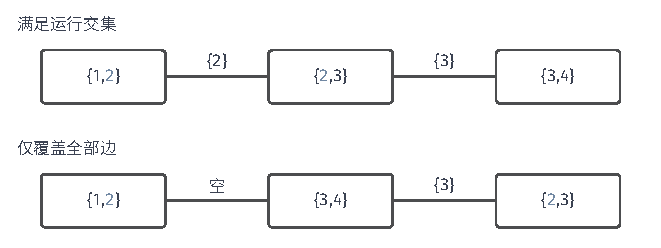
\includegraphics[width=112.0mm]{figures/01-mathematical-preliminaries-upper/07-graphs/tikz/graph-theory-running-intersection/figure.pdf}
  \caption{同一四顶点路径的两种袋连接。上行依次连接
  $\{1,2\},\{2,3\},\{3,4\}$，既覆盖边，又让每个变量的出现位置连通。
  下行同样覆盖全部边，却把含$2$的两个袋隔开，中间袋无法携带$2$的取值，因而不是树分解。}
  \label{fig:graph-theory-running-intersection}
\end{figure}

如图~\ref{fig:graph-theory-running-intersection}，仅覆盖顶点和边还不够：
在路径$1-2-3-4$上，若把两个含$2$的袋用不含$2$的袋隔开，两端就能分别取$z_2=0$和$z_2=1$
而沿途无从核对。运行交集保证一个变量的出现位置连成连通子树，
相邻接口上的一致性可以传到它的全部出现位置。

\paragraph{团作用域的整袋容纳}
树分解中任意一个团都整体包含在某个袋里，因此原始图中成团的高阶作用域能完整入袋。
其依据是树上的Helly性质：树上若干棵两两相交的连通子树必有公共顶点。
对团$C$，每个顶点$v\in C$出现的袋集合由运行交集保证是连通子树，
而边覆盖又使团内任意两点的子树两两相交，于是这些子树共有某个装下整个$C$的袋。
结构上能容纳仍不等于数值查询正确：因子还要唯一归属，组合与汇总规则由第~\ref{chap:graph-functions}章给出。

\subsubsection{顶点消元与填充}
想不再显式保留变量$v$，先要把所有含$v$的局部表的影响组织到剩余变量上。
图上的操作是：删除$v$前检查它当前的剩余邻居，必要时在邻居间补齐连接，再删去$v$及关联边。
新补的边称\term{填充边}（fill edge），它记录新表可能具有的联合索引，
不是原问题新增的独立约束；特殊函数有时仍可继续分解，袋给的是通用的作用域上限。

\subsubsection{分解宽度与树宽}
一个树分解的宽度是$\max_t|B_t|-1$，图的\term{树宽}（treewidth）是全部有效树分解宽度的最小值。
减$1$使含边的树可用父子二元袋得到宽度$1$，单顶点图宽度为$0$。
某次构造得到宽度$k$只给出“树宽不超过$k$”的上界；没有下界或最优性依据时，
不能把构造宽度直接称为该图的最小树宽。若每变量至多$q$个取值，
大小$k+1$的袋稠密表至多有$q^{k+1}$项，所以宽度控制的是同时索引的变量数，
而非自动保证任何任务都便宜。

\subsection{基于给定次序的补边分解法}

\paragraph{从消元接口构造袋的思想}
输入非空有限无向图和一个完整顶点次序$\pi$。记$N^+_\pi(v)$为删除$v$的当前填充图中
次序更晚的邻居（上标$+$表示次序后继，不是有向出邻域）。
每次删$v$前记录袋$B_v=\{v\}\cup N^+_\pi(v)$，把剩余邻居补成团，再删$v$。
\begin{algorithm}[给定次序补边分解]
  按$\pi$逐点读取当前剩余邻居并生成$B_v$；枚举这些邻居的无序对，只对缺失的边补入并记录；
  删除$v$及其当前关联边。每一步都从更新后的图重新读取邻居。
  全部袋生成后，$N^+_\pi(v)$非空时把$B_v$连到其中最早消去顶点$p(v)$的袋$B_{p(v)}$，
  为空时记为根袋；不同分量的根袋可用空交集边接成一棵袋树。
\end{algorithm}

\paragraph{父袋连接与运行交集}
父指针总指向次序更晚的点，所以袋连接不成环。原边由较早端点的袋覆盖；
若$z\in B_v$，邻居补团后$z$沿父袋一直保留到$B_z$，于是含$z$的袋连通，满足运行交集。
这就证明了下面的结构结论。

\begin{theorem}[消元序产生树分解]
  \label{thm:graph-theory-elimination-tree-decomposition}
  给定非空有限无向图的完整消元次序$\pi$，每步把剩余邻居补成团，
  则袋$B_v=\{v\}\cup N^+_\pi(v)$可连接成树分解，宽度不超过\term{诱导宽度}
  $k_\pi=\max_v|N^+_\pi(v)|$。因此树宽不大于任一消元次序的诱导宽度。
\end{theorem}

\paragraph{同图好坏次序的逐步比较}
在贯穿图上用$\pi=(1,4,2,3)$：$B_1=\{1,2,3\}$、$B_4=\{2,3,4\}$、$B_2=\{2,3\}$、$B_3=\{3\}$，
全程无新增边，最大袋大小$3$、宽度$2$。换$\pi'=(2,1,3,4)$：第一步$B_2$含全部四点，
必须补边$1-4$，后续袋为$\{1,3,4\},\{3,4\},\{4\}$，宽度升到$3$。
对应二值接口表分别有$4$项与$8$。两次构造都覆盖图，计算量却不同。

\begin{figure}[htbp]
  \centering
  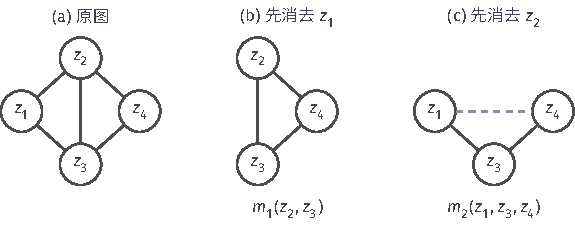
\includegraphics[width=97.282mm]{figures/01-mathematical-preliminaries-upper/07-graphs/tikz/graph-theory-elimination-fill/figure.pdf}
  \caption{两个首步消元产生不同接口。删去$z_1$后新表索引$(z_2,z_3)$；
  删去$z_2$后通常须索引$(z_1,z_3,z_4)$，紫虚线为填充边$1-4$。
  二值稠密接口表分别有$4$和$8$项。特殊函数可能还能分解，图给出的是通用作用域上限。}
  \label{fig:graph-theory-elimination-fill}
\end{figure}

\paragraph{结构代价与后续表计算}
令$d_t$为第$t$步的剩余邻居数，补边候选对共$\sum_t d_t(d_t-1)/2$，袋记录量为$\sum_t(d_t+1)$。
支持期望常数查边与更新的哈希邻接集合下，给定次序的结构操作期望时间约为
$O(n+m+\sum_t d_t^2)$，存储含原边、$F$条填充边及全部袋；稠密矩阵则占$O(n^2)$。
每变量至多$q$状态时，处理一袋的稠密表至多$q^{k_\pi+1}$项，输出接口表至多$q^{k_\pi}$项，
总时间还取决于袋数、因子数与每次运算成本。结构操作数与数值表的指数代价要分别报告。
树宽恰等于最优消元诱导宽度的完整双向证明不在本节展开；
实践中最小度、最少填充等启发式只给出可计算的上界。

\subsection{基于贪心次序选择的补边分解法}

没有给定$\pi$时，可以每轮先按某个局部评分选下一个点，再调用同一套补边、记袋、删除步骤。
\paragraph{用当前局部代价选下一点}
最小度规则比较当前剩余邻居数，最少填充规则比较该邻域中还缺多少对边，二者是不同评分。
\begin{algorithm}[贪心消元次序]
  对当前全部活跃点计算所选评分，以固定编号打破平局，取最低分点记入$\pi$并执行补边删除，
  然后在更新后的图上重新评分，直到图空。
\end{algorithm}
不能把按初始度数排一次序当作动态最小度，也不能用原图缺边数代替当前缺边数。

\paragraph{局部选择数例与代价边界}
贯穿图中$1,4$的度为$2$、填充评分为$0$，$2,3$的度为$3$且缺边$1-4$、评分$1$，
按编号先选$1$；余下$\{2,3,4\}$成团，再按编号得$(1,2,3,4)$，构造宽度仍为$2$。
每轮重算全部评分的直接版本，检查量可达$\sum_t\sum_{v\text{活跃}}(1+d_t(v)^2)$、最坏约$O(n^4)$；
采用缓存或优先队列前必须说明哪些边增删触发重算。局部评分没有最优树宽保证。

\section{弦图条件下的团树构造法}
\label{sec:graph-theory-chordal-elimination}

本节希望直接用原图的极大团作袋。先把极大团、弦图、完美消元序和团树分别讲清，
再给出无填充次序的构造与极大团的连接方法。

\subsection{极大团、弦图与团树的基本概念}

\paragraph{团、极大团与最大团}
一个团若不能再加入图中其他顶点而仍保持两两相邻，称为\term{极大团}；
“极大”按集合包含判断，要检查能否继续扩张，不是先比较大小。
顶点数在全部团中最多的称\term{最大团}。例如三角形$1,2,3$外加边$3-4$，
极大团是$\{1,2,3\}$和$\{3,4\}$，后者虽不可扩张却比前者小，不是最大团。
贯穿图的两个三点极大团$\{1,2,3\},\{2,3,4\}$恰好也都是最大团，但这只是特例；
团树方法需要全部极大团，不能只取最大的几个。

\paragraph{弦、弦图与弦化}
长度至少$4$的环上，连接两个在环上不相邻顶点的边称为该环的\term{弦}（chord），
按环上位置判断而不按画线内外判断。每个长度至少$4$的环都有弦的有限无向图称\term{弦图}
（chordal graph）；树没有环因而也是弦图，无对角边的四环不是弦图。
弦图的诱导子图仍是弦图。给原图补边直到成为弦图称\term{弦化}（chordal completion），
它改变输入图、可能改变原分离关系，补全图上的团树不等价于原图的全部查询。

\paragraph{单纯顶点与完美消元序}
当前邻居已经两两相邻的顶点称\term{单纯顶点}（simplicial vertex），删除它无需补边；
空邻域和单点邻域也算单纯，且必须检查当前余图而非初始邻域。
若按一个完整次序删点时每步的待删点在当前余图中都单纯，该次序称\term{完美消元序}
（perfect elimination ordering）。
\begin{definition}[弦图与完美消元序]
  \label{def:graph-theory-chordal-graph}
  有限无向图是弦图，当且仅当它具有完美消元序。
\end{definition}
其依据有两方面：每个非空有限弦图都有单纯顶点（非完全弦图甚至有两个不相邻的单纯顶点），
删去单纯点后诱导余图仍是弦图，故可反复删到图空；反之，若有无弦长环，
环上最早删除的点面对两个尚不相临的环邻居，不可能单纯，矛盾。
存在好次序不等于任意次序都好：贯穿图本是弦图，但先删$2$时其剩余邻居$1,3,4$不两两相邻，仍须补$1-4$。

\paragraph{团树}
以原图全部极大团为袋并满足运行交集的袋树称\term{团树}（clique tree）。
相邻团的交集保存共同变量：贯穿图两个极大团交集为$\{2,3\}$，团树边承载两变量接口，
但团树不决定接口表上做加法、取最大还是其他运算。图不连通时，不同分量的团可用空交集边接成一棵树。
有限非空弦图能由全部极大团构成团树，非弦图则不能无条件照搬这套原团构造。

\subsection{基于单纯顶点删除的完美序构造法}

\paragraph{无填充删除的思想}
与允许补边的消元不同，这里只选择当前邻居已经成团的点，因而全程不扩大剩余连接；
目标是输出一个完整无填充次序，或指出图不满足弦图条件。
状态为当前活跃点集、当前邻接和已输出次序，单纯性在每次删除后重新检查。

\begin{algorithm}[单纯顶点删除构造完美序]
  在当前活跃点中按固定编号找候选$v$，枚举其不同邻居$u,w$确认每对之间都有边
  （空邻域、单邻居直接合格）；找到合格点就追加到次序、保存当前邻域并删除$v$及关联边，
  在余图上重复直到图空。若非空余图找不到单纯点，返回“不满足弦图条件”及该余图，不暗中补边。
\end{algorithm}

\paragraph{四环补弦的算例核验}
对四环$1-2-3-4-1$，每个点的两个邻居都不相邻（$1,3$看到$\{2,4\}$缺边$2-4$，
$2,4$看到$\{1,3\}$缺边$1-3$），没有合格点，方法返回失败。
补入弦$1-3$后，$2$的邻居$\{1,3\}$已相连；删$2$后$1$的邻居$\{3,4\}$相连，再删$1$，
随后依次删$3,4$，得到$(2,1,3,4)$且全程无新增边。

\paragraph{输出次序的独立核验}
\begin{algorithm}[完美消元序核验]
  独立于构造过程，给原图和待检次序：先确认次序长度为$n$且恰含每个顶点一次；
  建立每点rank，对每个$v$取出原图中排名更晚的邻居$N^+_\pi(v)$，逐对检查其间是否有原边，全程不补边。
  发现缺边即返回$v$与该缺边对作为失败见证；全部通过才认证为完美消元序。
\end{algorithm}
复查$(2,1,3,4)$用于无弦四环时，首点$2$的更晚邻居$\{1,3\}$缺边，立即拒绝；
用于已补$1-3$的图才通过。直接重查的朴素构造邻接检查量最坏约$O(n^4)$、稠密存邻接占$O(n^2)$；
独立核验建rank与读邻接为$O(n+m)$，邻居对检查数为
$\sum_v|N^+_\pi(v)|(|N^+_\pi(v)|-1)/2$。两者职责不同，不应混为一项代价。

\subsection{基于团交集最大权树的接口构造法}

\paragraph{以共享变量连接团的思想}
输入弦图和已核验的完美序，要输出以全部极大团为袋、满足运行交集的接口树。
直觉上交集大的团应相连以携带更多共享变量，但任意接线不一定满足运行交集，
需要一条明确的最大总交集权规则。

\paragraph{从完美序生成极大团列表}
对每点生成$K_v=\{v\}\cup N^+_\pi(v)$，完美序保证各$K_v$是团；
删除重复集合和被其他$K$严格包含的集合，得到全部极大团。不遗漏的原因是：
任一团取其中最早消去的点，其余点都在该点剩余邻域中，整个团包含于某个$K_v$，
而各$K_v$本身是团，极大者恰为极大团。

\paragraph{建立交集权并选树边}
在$p$个团节点上建完全候选图，边权取$w(C,D)=|C\cap D|$，交集为空的零权边也保留。
\begin{algorithm}[最大交集权团树]
  把候选边按交集权从大到小排序，用并查集只接纳连接两个不同当前团分量的边，
  接满$p-1$条即停止（$p=1$时返回单个袋）；树边同时记录实际的接口集合。
\end{algorithm}
这与第~\ref{chap:graph-optimization}章的最大权生成树是同一种选边机制，其交换正确性在该章统一分析。

\begin{theorem}[最大权生成树与团树]
  \label{thm:graph-theory-clique-tree-maximum-weight}
  设$\mathcal H$为非空有限弦图，$\mathcal C$为其全部极大团，在以$\mathcal C$为节点的完全图上
  令$w(C,D)=|C\cap D|$（含零权边）。则候选图的一棵生成树满足运行交集，
  当且仅当它的总交集权最大。
\end{theorem}
直观理由是：对每个原顶点$v$，含$v$的$k_v$个团节点在树上至多需要$k_v-1$条两端含$v$的边
就能连成一片，等号成立恰当这些团连通；把所有顶点的这份计数相加就是总交集权，
而完美序构造出的团树能对每个顶点取等号，故最大权树恰满足运行交集。

\paragraph{贯穿图及四环的算例核验}
贯穿图极大团为$\{1,2,3\},\{2,3,4\}$，唯一候选边权$2$、接口$\{2,3\}$，
$2,3$在两端且经含它们的边相连。四环的极大团只是四条原边，
若要让每个顶点所属的两个边团都直接相连就需要四条连接而成环，选不出树，
所以不能给非弦四环的原团列表随便选一棵最大权树就宣称满足运行交集。
给定弦图上连接团、为原图选弦化、在所有补边中找最小宽度是三件不同的任务；
交集权计算、排序及包含筛选的代价也要随团数与集合表示另行计入。

\section{基于祖先道德化的d-分离判定法}
\label{sec:graph-theory-directed-transformations}

第~\ref{chap:graph-paths}章定义了活跃路径与d-分离，但逐条枚举全部底层路径代价高且容易遗漏。
本节把一次条件分离查询等价地转换成一张临时无向图上的可达查询。

\paragraph{条件分离查询的输入与\term{祖先闭包}}
输入有限DAG和两两不交、$A,B$非空的集合$A,B,S$，判定给定$S$时$A,B$是否d-分离。
集合$W$的祖先闭包
\[
  \operatorname{An}(W)=W\cup\{v:\text{存在从}v\text{到}W\text{中某点的有向路径}\}
\]
显式包含$W$自身；本次查询取$W=A\cup B\cup S$。祖先闭包要在入邻接表上逆向BFS/DFS求得。

\paragraph{诱导\term{祖先图}、骨架与\term{道德图}}
在祖先闭包$U$上取诱导图$\mathcal G[U]$，保留$U$内部全部原弧——先限定点集再补边，
次序不可交换。有向图的骨架只是去掉弧方向、保留原有邻接。
\term{道德化}（moralization）则先把每个顶点的不同父节点两两相连、再去掉全部方向，
新增的父点边是它与骨架的区别；这里只对诱导祖先图道德化。

\begin{definition}[骨架、祖先闭包与道德图]
  \label{def:graph-theory-directed-structure}
  骨架$\operatorname{skel}(\mathcal G)$是同顶点集的无向图，$i,j$相邻当且仅当
  $i\to j$或$j\to i$存在。祖先闭包$\operatorname{An}(W)$如上定义，
  $\mathcal G[\operatorname{An}(W)]$为诱导祖先图。道德图$\operatorname{mor}(\mathcal G)$
  把每个顶点的任意两个不同父节点连成无向边后再去掉所有弧方向；
  若每个父集在骨架中原本已两两相邻，称该DAG为\term{完美有向图}。
\end{definition}

\paragraph{逆向检索到无向分隔的五步实现}
\begin{algorithm}[祖先道德化d-分离判定]
  第一步，以$A\cup B\cup S$为多源在入邻接表上逆向遍历，得到祖先闭包$U$（保留种子本身）；
  第二步取诱导图$\mathcal G[U]$；第三步只在该诱导图内，把每个顶点的父集无序对补边并去掉全部方向，
  得到本次查询的无向道德图；第四步删除$S$及关联边；第五步从$A$的所有点同时BFS，
  检查能否到达$B$：能到达则不d-分离，否则d-分离，并可沿前驱输出查询图中的一条路径。
\end{algorithm}
其等价性依据是：给定$S$时原图的一条活跃路径，其碰撞点都在$S$的祖先中、
其余内部点都是端点或$S$的祖先，故整条路径落在诱导祖先图里，
用道德边绕过属于$S$的碰撞点便得到避开$S$的无向路径；反过来，道德图中避开$S$的路径
把每条新增道德边展开回$u\to c\leftarrow v$，必要时沿有向路径改道，也能还原出一条活跃路径。
这里只使用该判据与操作次序，完整的路线去重证明不在主线展开。查询图里沿道德边走的路线
不是原图中顺箭头的有向路径。

\begin{figure}[htbp]
  \centering
  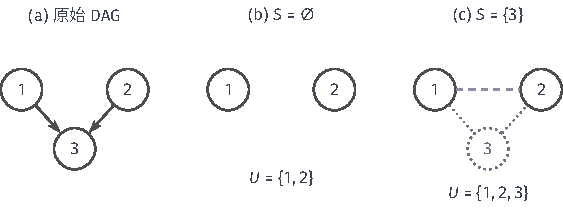
\includegraphics[width=95.282mm]{figures/01-mathematical-preliminaries-upper/07-graphs/tikz/graph-theory-ancestor-moral-query/figure.pdf}
  \caption{祖先道德图随查询条件改变。端点固定为$1,2$；空条件集时查询图只有两个孤立顶点。
  给定$3$时，扩大的祖先集合使道德化加入新增边$1-2$，删除条件点$3$后这条边仍在。
  不能先道德化整图再取查询顶点。}
  \label{fig:graph-theory-ancestor-moral-query}
\end{figure}

\paragraph{碰撞及另一条通路的逐步查询}
如图~\ref{fig:graph-theory-ancestor-moral-query}，在$1\to3\leftarrow2$上取$A=\{1\},B=\{2\}$：
空条件时祖先闭包只有$\{1,2\}$，诱导图没有$3$、不补$1-2$，两点不连通，判为d-分离；
$S=\{3\}$时闭包含三点，父集$\{1,2\}$促使道德化补$1-2$，删$3$后边仍在，判为不分离。
若另有$3\to d$，给定后代$d$也会经祖先闭包得到同样结果。若先对整图道德化再截取$\{1,2\}$，
会错误留下$1-2$，说明“先取祖先、后道德化”的次序不能交换。
此外即使碰撞路径在空条件下关闭，若另有链$a\to e\to b$，$a,b$仍不分离：
阻断一条路径不足以确认分离。

\paragraph{代价、表示与查询边界}
建入邻接与逆向祖先检索为$O(n+a)$。道德化要枚举诱导图中每个父集的点对，
共$\sum_v p_v(p_v-1)/2$对，点的父集很大时即使原图稀疏、查询图也可能接近稠密，
不能把整步统称$O(n+a)$；用稠密掩码存边另占$O(n^2)$。每次$A,B,S$变化都可能改变祖先集和新增边，
输出的是这一次查询的临时等价无向图，不自动给出一张保留全部条件查询的固定图，
从图分离到概率独立仍需第~\ref{chap:graph-paths}章说明的分解假设。

\section{本章小结}

\paragraph{访问次序与查询输出}
BFS给出边数层和一条发现路线，DFS给出当前分支、回边见证与完成信息；
Kahn与DFS逆完成序在DAG上构造处理次序。需要什么输出决定保存什么状态，
任一遍历次序都不能直接当作最短路线或拓扑序。连通标记、两遍标签合并和种子队列重建
复用同一套邻接检索，但分别输出全部分量或指定可达集，$4/8$邻接、掩模范围、
结构元方向和空种子条件都随方法固定。

\paragraph{分解的作用与代价}
父边提取保留分量连通却可能改变距离和分隔；给定分隔集把共享变量保留为接口，
消元补边再把潜在作用域组织成袋，宽度控制同时索引的变量数。
运行交集约束变量取值能否沿接口核对，因子唯一归属约束数值不被重复计入，二者缺一不可。
次序会改变填充与最大袋规模；单纯顶点删除在弦图条件下给无填充记录，
团交集最大权树再连接全部极大团，它们都有具体输入与构造代价，不因其名称就成为线性或最优。

\paragraph{单次分离查询与后续计算}
祖先道德化按“逆向求祖先—取诱导图—补父点边—删条件点—无向检索”五步完成一次d-分离判定，
查询图随$A,B,S$而变。本章产出的是访问次序、标签、连接骨架、局部袋和判定结果；
第~\ref{chap:graph-optimization}章在相应结构上加入路径、流量、生成树等优化目标，第~\ref{chap:graph-functions}章在合法运算下组合、汇总配置表。
结构可用、目标最优与数值查询正确，是需要分别建立的三件事。

\chapter{图上的约束优化}
\label{chap:graph-optimization}

前面两章分别回答了“图上有什么关系”和“怎样检索、分解这些关系”。本章在同一类离散结构上
加入目标与约束，研究怎样作选择。在同一张交通网络上，选最短路线、分配各弧流量、
铺一条最省线的连通网络，会得到不同答案：前者选一条路径，流量给各条弧分配数值，
生成树则选一组边。边旁的数字是长度、容量还是建造成本，必须由问题先指定，
方法的正确性依赖它的用途。

本章按选择对象分六类方法。最短路在端点约束下选路线；距离变换同时求多个位置到目标集的距离；
最大流在容量约束下分配各弧流量；最小生成树在连通约束下选连接边；匹配与指派在互斥约束下
两两配对；标记与划分则为每个顶点选离散标签。每类方法都先说明维护什么可行状态，
再说明哪条递推、交换或上下界证据排除了更好的候选，最后交代代价与失效条件。
涉及一般图时记$n=|V|$、无向边数$m$、有向弧数$a$，默认以邻接表访问并另存边的长度、容量或成本。

\section{基于递推与松弛的最短路方法}

以下加权算法统一在有向图上表述，边长为有限实数；无向边可换成两条同长度反向弧，
因此无向负边来回经过就形成负的闭行走。令$\mathcal P_{s,v}$为$s$到$v$的简单路径集合，
$\mathcal W_{s,v}$为允许重复顶点、边的全部有限行走集合，两个目标分别是
\[
  d_{\mathrm{path}}(s,v)=\min_{P\in\mathcal P_{s,v}}\ell(P),\qquad
  d_{\mathrm{walk}}(s,v)=\inf_{W\in\mathcal W_{s,v}}\ell(W),
\]
空候选集约定为$+\infty$。可达时简单路径只有有限条，最小值存在；行走候选可无限。
标准单源算法求的是$d_{\mathrm{walk}}$：若不存在从$s$可达的负环，真实距离$D(v)$满足
\begin{equation}
  D(s)=0,\qquad
  D(v)=\min_{u\to v}\{D(u)+\ell_{u,v}\}\quad(v\neq s),
  \label{eq:graph-theory-shortest-path-bellman}
\end{equation}
空前驱的最小值取$+\infty$。但这组等式本身不唯一确定距离：
$s\to a$长$5$、$a\leftrightarrow b$两弧长$0$时，任何$D(a)=D(b)\leq5$都满足局部等式，
实际距离却是$5$。所以算法必须从“源为零、其余为无穷”的标签出发，并保存实际路线见证。
下面三种一般方法按可用的结构区分：DAG靠拓扑序一遍完成，Bellman--Ford允许反复修正，
Dijkstra在非负边长下永久确定标签；编辑距离与DTW则是DAG状态递推的两个专门应用。

\subsection{DAG拓扑递推法}

DAG中到达一个顶点的全部前驱都能先算完，标签此后不再被修正。
初始化$L(s)=0$、其余$+\infty$、前驱为空，按一个拓扑序访问$u$，对每条出弧$u\to v$用候选
$L(u)+\ell_{u,v}$松弛：严格更小时更新$L(v)$与$p(v)$。
\begin{algorithm}[DAG拓扑递推最短路]
  先求一个拓扑序；按序处理每个顶点，处理$v$时它的所有入邻居都已处理完毕，
  松弛其全部出弧。终点标签有限时沿前驱逆序恢复路径。
\end{algorithm}
对拓扑序归纳：每条到达$v$的非空路径以某条$u\to v$结束，其前缀成本不小于已求出的$L(u)$，
而每个有限标签又都有实际路径见证，两个方向夹定最小值。
拓扑排序与扫描全部弧共$O(n+a)$，额外$O(n)$。这里允许负边，
因为正确性依赖无环次序，而不依赖“路径前缀比整条路径短”。

在四点DAG（$s\to a$长$2$，$s\to b$长$5$，$a\to b$长$-1$，$a\to t$长$5$，$b\to t$长$2$）上，
按$(s,a,b,t)$：处理$s$得$a=2,b=5$；处理$a$把$b$改为$1$、$t$改为$7$；
处理$b$把$t$改为$3$，恢复路径$s\to a\to b\to t$。

\paragraph{编辑距离的网格递推（扩展）}
同一个“无环状态网格”还可由两条序列的前缀长度构造。令$E(i,j)$为把序列$a$的前$i$个元素
改成序列$b$前$j$个元素所需的最少单元素插入、删除、替换次数。最后一步只有三类：
删$a_i$、插$b_j$、末元素匹配或替换，故
\begin{equation}
  E(0,j)=j,\quad E(i,0)=i,\qquad
  E(i,j)=\min\bigl\{E(i-1,j)+1,\ E(i,j-1)+1,\
    E(i-1,j-1)+\mathbb I_{\{a_i\neq b_j\}}\bigr\}.
  \label{eq:graph-edit-distance-recursion}
\end{equation}
每条状态边都使$i+j$增加，所以这是DAG上的最短路，$E(m,n)$即\term{Levenshtein编辑距离}。
对$(A,B)$与$(A,C,B)$，三行四列分别为$(0,1,2,3)$、$(1,0,1,2)$、$(2,1,1,1)$，
沿“匹配$A$—插入$C$—匹配$B$”得距离$1$。全表连同前驱为$O((m+1)(n+1))$时间与存储，
只求值时用两行可降到$O(n+1)$空间；字符还是词为计数单位须先固定，
相邻交换不设为一次操作，树编辑还需另行规定层级规则，不能展平成字符串套用同一距离。

\paragraph{\term{动态时间规整}（扩展）}
两序列以不同速度经历同一过程时，要让一侧一个读数对应另一侧多个读数。
令局部差异$c(i,j)\geq0$，对齐路径从$(1,1)$到$(m,n)$，每步取$(1,0),(0,1),(1,1)$，则
\begin{equation}
  D(i,j)=c(i,j)+\min\{D(i-1,j),D(i,j-1),D(i-1,j-1)\},\quad D(0,0)=0,
  \label{eq:graph-dtw-recursion}
\end{equation}
正下标的边界行列取$+\infty$，强制两端都参与全局对齐，所以恰一条序列为空时不可行，
不能照搬编辑距离的有限边界。对$a=(1,2)$、$b=(1,1,2)$取绝对值差，
路径$(1,1),(1,2),(2,3)$成本为零；不同长度序列可能零成本，故DTW不自动满足度量公理。
带宽约束$|i-j|\leq w$在$|m-n|>w$时连终点都排除；要最小化平均成本须把路径长度纳入目标，
不能把最小总成本事后除以长度。

\subsection{Bellman--Ford松弛法}

有环时前驱距离可能在以后下降，一遍更新不够。令$L^{(0)}(s)=0$、其余为$+\infty$，
每一轮右侧全部读取上一轮标签：
\[
  L^{(k)}(v)=\min\Bigl\{L^{(k-1)}(v),\
    \min_{u\to v}\bigl(L^{(k-1)}(u)+\ell_{u,v}\bigr)\Bigr\}.
\]
\paragraph{同步松弛的状态与逐轮更新}
\begin{algorithm}[同步Bellman--Ford]
  每轮复制上一轮标签，逐弧用上一轮值计算候选并取最小；重复至多$n-1$轮，
  若一整轮没有任何更新可提前停止。需要路线时连同轮次一起记录前驱。
\end{algorithm}
可归纳证明$L^{(k)}(v)$恰为至多$k$条边到达$v$的最小行走成本：
$k=0$只有源的零步行走，下一轮候选由旧行走或旧前缀加末弧组成。
在上面的四点DAG上逐轮标签为$(0,\infty,\infty,\infty)$、$(0,2,5,\infty)$、
$(0,2,1,7)$、$(0,2,1,3)$。

\paragraph{轮数上界与就地更新}
不受可达负环影响的目标，其行走可删去非负闭合段，最短见证至多$n-1$条边，故$n-1$轮足够。
常用的就地更新在一轮内提前传播新值，此时“恰为至多$k$边最优”的解释只属于同步版本，
但因仍覆盖全部候选且标签都有路线见证，轮数上界不变。

\paragraph{负环种子与后继标记}
完成$n-1$轮后固定标签，再检查所有满足$L(u)<+\infty$且$L(u)+\ell_{u,v}<L(v)$的弧，
把其终点作为种子，并沿出弧遍历种子的全部后继，标为$-\infty$。
正向看，种子有一条比全部至多$n-1$边行走更优的至多$n$边行走，其中必含重复顶点且含负环；
反向看，任一从源可达的负环若环上没有可改善弧，沿环把不等式相加会得到$0\leq\ell(\text{环})<0$的矛盾。
所以标记的恰是“从源可达负环、且该环能继续到达”的目标。
\begin{figure}[!htb]
  \centering
  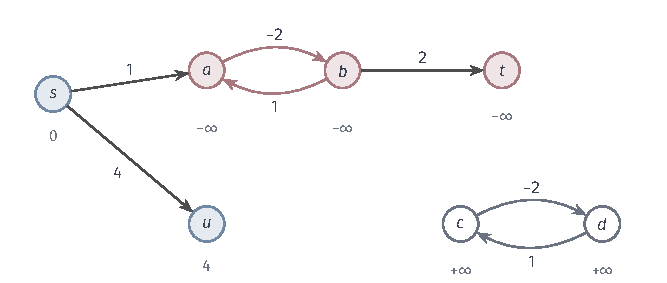
\includegraphics[width=112mm]{figures/01-mathematical-preliminaries-upper/00-shared/tikz/graphs-and-signals-comprehension-additions/graph-negative-cycle-reach.pdf}
  \caption{三种距离状态同处一图。可达负环上的$a,b$及其后继$t$行走下确界为$-\infty$；
  未回接旁支$u$距离有限（$4$）；与$s$不连通的负环$c,d$不影响本次单源查询，距离为$+\infty$。}
  \label{fig:vol1-add-graph-negative-cycle-reach}
\end{figure}
如图~\ref{fig:vol1-add-graph-negative-cycle-reach}，受影响的$-\infty$、
旁支有限距离、不可达$+\infty$要分别报告。同步实现保守时间为$O(n(n+a))$、
状态$O(n)$；若保存全部轮次前驱以回溯有限见证，需$O(n^2)$条记录，
负无穷目标只给负环证据、不可达点无路径。

\subsection{基于贪心选择的Dijkstra法}

若边长全部非负，就能每次永久确定一个顶点，因为到未确定点的更远路线无法靠后半程把成本降下来。
\begin{algorithm}[Dijkstra]
  初始化$D(s)=0$、其余$+\infty$、已确定集为空，把源放入按距离排序的优先队列。
  每次取暂定距离最小的未确定点$u$，永久确定它，再用$D(u)+\ell_{u,v}$松弛其出邻居，
  改善时更新距离、前驱并降键（或重复插入、出队时跳过过期条目）；队列空结束。
\end{algorithm}

\begin{theorem}[Dijkstra算法的贪心正确性]
  \label{thm:graph-theory-dijkstra-correctness}
  若全部边长非负，则顶点$u$被选入已确定集合时，其暂定距离$D(u)$
  等于从$s$到$u$的行走下确界，也等于简单路径最小值。
\end{theorem}
\begin{proof}
有限暂定标签都来自实际路线，故$D(v)\geq D_{\text{真}}(v)$。假设此前确定的点都正确，
考虑新选入的$u$。若有更短路径，取其上第一个未确定点$y$及其已确定前驱$x$，
松弛给出$D(y)\leq D(x)+\ell_{x,y}$，不超过该路径到$y$的前缀；
剩余边长非负使前缀不超过整条路径，而最小键选择又给$D(u)\leq D(y)$，矛盾。
最小键为无穷时尚有可达点也会与“跨出已确定集的第一条边必产生有限标签”矛盾，故这些点确不可达。
\end{proof}
非负性恰用在“前缀代价不超过全路径”这一步。索引二叉堆支持$O(\log n)$取最小与降键，
邻接表下总时间$O((n+a)\log n)$、额外$O(n)$。
在前面的非负四点图上依次确定$a=2$、$b=3$、$t=5$。
反例$s\to a$长$2$、$s\to b$长$5$、$b\to a$长$-4$中没有负环，
算法仍会先把$a$误定为$2$（真实距离$1$），所以条件必须针对机制核验。

\section{基于多源传播与下包络的距离变换方法}

有时要为每个位置求到某个目标集合$F$的距离$D(p)=\min_{q\in F}d(p,q)$（空$F$取$+\infty$）。
先固定$d$是沿邻接行走的路径长度还是直接按坐标差定义的距离；障碍会影响前者而不影响后者。

\subsection{多源BFS传播法}
单位边长时把所有目标位置同时置零、入队，其余为$+\infty$，BFS分层证明原样适用：
首次发现距离就是到任一目标的最少边数，并给一条见证。
在一维位置$0$至$4$、目标$\{0,4\}$上，初始队列$[0,4]$，逐层得到距离$(0,1,2,1,0)$。
非负加权边改用多源Dijkstra（所有源同时为零），不能用FIFO首次发现就定值。
一般邻接表为$O(n+m)$，$P$个位置的规则网格为$O(P)$。

\subsection{双向扫描法}
无障碍矩形的4邻接距离可两遍扫描：正向（上到下、左到右）用上、左邻居加一取小，
反向用下、右邻居加一取小。任一源—终点的曼哈顿最短路都可在矩形内选一个转折点，
拼成一段右/下步加一段左/上坡，故两遍已覆盖最优见证、不会低估，总时间$O(P)$；
有障碍时路线可能多次换向，该保证失效。
轴向步成本$a$、对角步成本$b$，在$0<a\leq b\leq2a$且无障碍时，
最短成本为$b\min(|\Delta i|,|\Delta j|)+a\bigl||\Delta i|-|\Delta j|\bigr|$。
取$a=3,b=4$得常用\term{倒角距离}，归一化后对角为$4/3$而非$\sqrt2$，
所以它是该图上的精确路径距离，却不是精确欧氏距离。

\subsection{一维二次下包络法}
\label{sec:graph-quadratic-distance}
要精确计算平方欧氏距离，可把目标写成$q\in F$时$f(q)=0$、其余$+\infty$，
再最小化$f(q)+a(x-q)^2$。先研究一维问题
\begin{equation}
  \mathcal D(x)=\min_{q=0,\ldots,n-1}\{f(q)+a(x-q)^2\},\qquad a>0,
  \label{eq:graph-quadratic-distance-transform}
\end{equation}
其中$f$也可取任意有限实数（此时结果可能为负，不必是距离）。
直接枚举需$O(n^2)$，但所有候选是曲率相同的抛物线，只需保留某处可能最低者。
对中心$p<q$，消去共同的$ax^2$项，两曲线唯一交点为
\begin{equation}
  s(p,q)=\frac{f(q)+aq^2-f(p)-ap^2}{2a(q-p)}.
  \label{eq:graph-parabola-intersection}
\end{equation}
交点右侧较大中心$q$更低，故随输出坐标增大，最低候选的中心只向右移。
\begin{algorithm}[抛物线下包络]
  维护候选中心栈$v_0,\ldots,v_k$及各自开始占优的位置
  $z_0=-\infty<z_1<\cdots<z_k$，以$+\infty$收尾。跳过全部$f$为无穷的候选；
  新中心$q$入栈前求它与栈顶的交点$s$，若$s\leq z_k$说明旧栈顶已被全面压低，弹出后重算，
  直到$s>z_k$再压入。建栈后用只向右移动的指针按整数$x$选覆盖当前位置的候选求值。
\end{algorithm}
每个中心至多入栈、出栈一次，查询指针只前进，总时间与存储均为$O(n)$。
$f(0)=f(4)=0$、其余无穷时两抛物线交于$2$，输出$(0,1,4,1,0)$；
加入$f(1)=10$的短例可看到中间候选被弹出，结果与逐候选取最小一致。

\subsection{逐轴二次距离变换法}
二维（及高维）二次成本各轴项不混合，可逐层换序：
\[
  \min_{q_1,q_2}\{f(q_1,q_2)+a_1(p_1-q_1)^2+a_2(p_2-q_2)^2\}
  =\min_{q_2}\Bigl\{a_2(p_2-q_2)^2+
    \min_{q_1}[f(q_1,q_2)+a_1(p_1-q_1)^2]\Bigr\}.
\]
先沿第一轴对每条直线跑一维变换，中间数组再沿第二轴跑，$d$维$P$个位置共$O(dP)$；
保存最近源时要把前一轴的源索引带到后一轴。$a_j=1$且$f$为零/无穷指标时输出平方欧氏距离，
最后逐点开方才是欧氏距离：$\{0,4\}$的平方输出$(0,1,4,1,0)$开方为$(0,1,2,1,0)$。
最大化“响应减二次惩罚”时令$f=-R$再取反；线性位移项可分别并入输入与输出，
但含两轴混合乘积的成本一般不能逐轴分离。

\section{基于残量增广的最大流方法}

这次不是选一条路线，而是在多条路线可并行、每条弧又有通过上限时共同分配流量。
两条共用容量$1$的首弧的路线合计至多送$1$，不能各送$1$。
固定有限有向网络与不同端点$s,t$，每条弧有有限非负容量$c_{i,j}$，
非弧按容量$0$延拓（这些零条目不是新通道）。一个\term{流}（flow）$f$满足
\[
  0\leq f_{i,j}\leq c_{i,j},\qquad
  \sum_{u:u\to v}f_{u,v}=\sum_{w:v\to w}f_{v,w}\quad(v\neq s,t),
\]
即容量约束加内部流守恒。流值$|f|$是源净流出；对内部守恒式求和可知它等于汇净流入，
不是全图弧流量之和。取$s\in S,t\notin S$，割容量为
$c(S,V\setminus S)=\sum_{i\in S,j\notin S}c_{i,j}$，只计源侧跨向汇侧的容量。
对$S$内部守恒求和可知任意流值不超过任意割容量。

\subsection{残量增广法}
已选路线可能抢占更好安排，所以要能撤回。对每条原弧$i\to j$建立容量$c_{i,j}-f_{i,j}$的正向残量弧
（可追加）和容量$f_{i,j}$的反向残量弧（可撤回），只保留正容量残量弧，并保留原弧身份；
撤回不要求原网络真有$b\to a$通道。原弧容量$3$、已发$2$时，正向残量$1$、反向残量$2$。

\begin{algorithm}[残量增广最大流]
  从零流开始；在当前残量网络搜索$s$到$t$的路径，没有则停止；
  取路径上最小残量$\delta$为瓶颈，沿正向残量把对应原流加$\delta$、沿反向残量减$\delta$；
  更新残量后重复，结束时输出流以及残量网络中从$s$可达的集合$S$。
\end{algorithm}
瓶颈保证不超容量、不为负，路径内部流入流出变化抵消，源净流出严格增加$\delta$。

\begin{theorem}[最大流最小割定理]
  \label{thm:graph-theory-max-flow-min-cut}
  在有限非负容量网络中，最大$s$--$t$流值等于最小$s$--$t$割容量。
\end{theorem}
\begin{proof}
可行流由有限个闭有界线性约束定义、含零流，故最大流$f$存在。若其残量网络还有$s$--$t$路径，
按上法增广得到更大流，矛盾。取残量网络中$s$的可达集$S$，则跨出$S$的原弧必已满流
（否则可沿正向残量离开），从外面流入$S$的原弧必为零流（否则可沿反向残量离开），
于是$|f|$恰等于割容量$c(S,V\setminus S)$。任意流不超过任意割，故此流与此割分别最优。
\end{proof}

\begin{figure}[htbp]
  \centering
  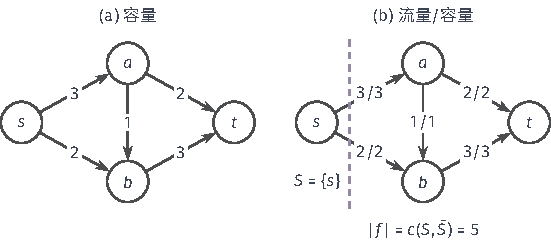
\includegraphics[width=93.282mm]{figures/01-mathematical-preliminaries-upper/07-graphs/tikz/graph-theory-flow-cut-certificate/figure.pdf}
  \caption{同值流与割构成最优性证书。跨出$S=\{s\}$的容量为$3+2=5$，等于实现的流值；
  图中画原网络弧，不画残量反向弧。}
  \label{fig:graph-theory-flow-cut-certificate}
\end{figure}

整数容量下从零流每次增广整数瓶颈，流始终为整数、每次至少增$1$，
源出容量和$C_s$有限，故至多$C_s$次增广终止，也证明了整数最优流存在；
这个次数依赖容量数值，不是位长多项式。容量取$3,2,1,2,3$时
依次沿$s\to a\to t$、$s\to b\to t$、$s\to a\to b\to t$增广$2,2,1$得流值$5$，
割$\{s\}$容量也是$5$（图~\ref{fig:graph-theory-flow-cut-certificate}）。
单位容量网还能演示撤回：首次沿$s\to a\to b\to t$后，第二次借残量$b\to a$改道，
最终真实路线为$s\to a\to t$与$s\to b\to t$。线性搜索残量路的基本实现时间为
$O((C_s+1)(n+a))$；任意实容量下紧性保证最优流存在，却不保证任意选路有限终止。

\section{基于安全选边的最小生成树方法}
\label{sec:graph-theory-minimum-spanning-tree}

每条无向边附带建造成本时，要在覆盖全部顶点、连通且无环的边集中选总成本最小者，
即\term{最小生成树}（minimum spanning tree, MST）。它最小化的是连接全网的建造费用，
不保证树上距离等于原图最短路：三角形边长$2,2,3$时MST费用$4$，原长$3$直连的两点在树上距离变为$4$。

对非平凡割$(S,V\setminus S)$，跨割成本最小的边称轻边。
\begin{lemma}[最小生成树的割性质]
  \label{lem:graph-theory-mst-cut-property}
  若边集$A$已包含在某棵MST中，且某割不切断$A$的任何边，则该割的一条轻边$e$
  可与$A$一起包含在某棵MST中。
\end{lemma}
\begin{proof}
取包含$A$的MST $T$。若$e\notin T$，加入$e$形成唯一环，环上必有另一条跨割边$f$才能回到原侧；
轻边给$w_e\leq w_f$，删$f$得到的生成树$T+e-f$成本不增，且因割未切$A$而$f\notin A$，
新树仍含$A$与$e$。
\end{proof}
负成本不影响这个相对比较；平局可产生多棵MST，但最小总成本唯一。

\subsection{Kruskal分量合并法}
\begin{algorithm}[Kruskal]
  先为每个顶点建单元并查集类，把全部边按成本（并列时按固定边序）排序；
  逐条取边$(u,v)$，若find代表相同则跳过（加入会成环），否则选中该边并union两类、分量数减一；
  连通图选满$n-1$条即停止，否则输出最小生成森林并报告不连通。
\end{algorithm}
在五点七边图（$ab=1,bc=2,cd=3,ac=4,bd=5,ce=6,de=7$）上，
依次接纳$ab,bc,cd$（此时$\{a,b,c,d\}$与$\{e\}$两类，累计$6$），
$ac$、$bd$因成环跳过，接纳$ce$后全连通，所选边为$\{ab,bc,cd,ce\}$，成本$12$。
接纳边之所以安全，是因为取其一端当前分量作割时，所有更轻边都已处理、不可能还跨此割，
当前边正是轻边。排序$O(m\log m)$，并查集在路径压缩加按秩合并下摊还$O(m\alpha(n))$。

\subsection{Prim单树扩展法}
\begin{algorithm}[Prim]
  固定起点$a$，维护一个已连通集$S$，为每个外部点$v$保存键
  $\operatorname{key}(v)=\min_{u\in S}w_{u,v}$及对应父点；
  反复取键最小的未加入点$u$加入$S$、把其父边收入树，并用$u$的邻边松弛外部点的键（用索引堆降键），
  直到$S$覆盖该分量。
\end{algorithm}
键是一条跨割边的成本，不是Dijkstra的累计路线长度。
在同一五点图上从$a$开始：先取$ab$（键$1$），$b$把$c$的键从$4$改为$2$、$d$设为$5$；
取$bc$后$d$改为$3$、$e$设为$6$；取$cd$后检查$de=7$不优于$e$的$6$；最后取$ce$，
得到同样四条边、成本$12$。每次最小键恰是割$(S,V\setminus S)$的轻边，割性质逐步保证可扩成MST。
索引堆下$O((n+m)\log n)$，朴素数组选最小为$O(n^2+m)$。
从$e$出发会先取$ec=6$再取$cb=2,ba=1,cd=3$，说明Prim的选边成本不必递增，
与Kruskal全局排序的思想不同；非连通图逐分量求森林。
另外，第~\ref{chap:graph-traversal}章团树构造在团候选图上求最大总交集权，把比较改为取最大即可复用同一交换机制，
但其运行交集保证来自团树定理，不是贪心本身给出的。

\section{基于交替增广的匹配与指派方法}

二部图$\mathcal G=(U,W,E)$的\term{匹配}（matching）是一组不共享端点的边。
不能再加边的称极大匹配，边数最多的才称最大匹配——局部加不进边，
仍可能靠替换已有边扩大配对。先最大化配对数量，再在“每个左对象都必须配对”的要求下最小化成本。

\subsection{交替路径增广匹配法}
建一个网络：源到每个$u\in U$连容量$1$弧，每条候选边改容量$1$弧$u\to w$，
每个$w\in W$再连容量$1$弧到汇。任一匹配对应一个同值整数流；
源、汇两侧的单位容量保证每个左右点至多选一次，故整数最大流的值恰为最大匹配的边数，
不能用分数阈值化代替实际配对。
匹配的\term{增广路径}两端都是未匹配点，路径上未选边与已选边交替出现；
沿路径翻转后内部点仍各有一条匹配边，两端各添一条，匹配数增加$1$。
它正是该单位容量网络的残量$s$--$t$路径：未匹配边正向走、已匹配边反向撤回。
如图~\ref{fig:graph-theory-matching-augmentation}，已有$\{a-x,b-y\}$时，
自由点$c$沿$c-y-b-z$搜索，撤$b-y$、加$c-y$与$b-z$，得到大小$3$的匹配。
无增广路径即无残量路径，由最大流最小割得最大性证书。
\begin{figure}[htbp]
  \centering
  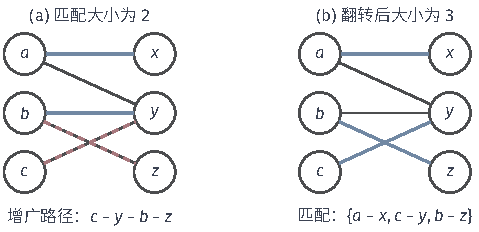
\includegraphics[width=81.188mm]{figures/01-mathematical-preliminaries-upper/07-graphs/tikz/graph-theory-matching-augmentation/figure.pdf}
  \caption{沿交替路径$c-y-b-z$重排匹配：撤去$b-y$，加入$c-y,b-z$，保留$a-x$，
  配对数由$2$增为$3$。连线表示候选配对，不表示因果方向。}
  \label{fig:graph-theory-matching-augmentation}
\end{figure}
一般含奇环的非二部图不能用这套左右流构造；加权匹配目标也不同，需另建机制。

\subsection{匈牙利\term{紧边}增广法}
\label{sec:graph-weighted-assignment}
设左侧$m$个对象都须分到右侧$n\geq m$个不同对象，允许边成本为有限实数$c_{ij}$，
\begin{equation}
  \min_x\sum_{i,j}c_{ij}x_{ij},\qquad
  \sum_jx_{ij}=1,\quad \sum_ix_{ij}\leq1,\quad x_{ij}\in\{0,1\}.
  \label{eq:graph-rectangular-assignment}
\end{equation}
补$n-m$个零成本虚拟左对象可化为$N=n$阶方阵完整指派（每行每列恰选一条），虚拟对象只占用未用列。
若允许真实对象不匹配，不能只把等式改成不等式（非负成本下空匹配会最优），
而要为每个左对象设成本$\rho_i$的专属虚拟列、每个右对象设成本$\eta_j$的专属虚拟行，
非专属真实—虚拟配对禁配，使总成本恰为配对成本加未匹配惩罚。

给每行、每列选\term{指派势}$u_i,v_j$，使每条允许边满足
\begin{equation}
  u_i+v_j\leq c_{ij};
  \label{eq:graph-assignment-potentials}
\end{equation}
任何完整指派的成本都不小于$\sum_i u_i+\sum_j v_j$（每行每列恰计一次）。
取等号的边称紧边；若能只用紧边完成完整指派，其成本恰等于该下界，即全局最优，
这同时证明对应的线性松弛有整数最优解。
\begin{algorithm}[匈牙利紧边增广]
  取$u_i=\min_j c_{ij}$、$v_j=0$建初始可行势；维护紧边匹配，反复从一个自由行出发
  沿“紧的未匹配边到列、已匹配列沿其匹配边回行”建交替树。到达自由列就翻转增广；
  若树被卡住，令$S,T$为树中行、列，取$\delta=\min_{i\in S,j\notin T}(c_{ij}-u_i-v_j)$，
  把$S$中行势加$\delta$、$T$中列势减$\delta$，保留可行性与已有紧匹配并至少新增一条紧边，
  再继续，直到全部行匹配。
\end{algorithm}
对成本矩阵$\begin{bmatrix}1&2\\1&100\end{bmatrix}$，逐行贪心得$101$；
初始势$u=(1,1),v=(0,0)$，从第二行建树得$\delta=1$，调势至$u=(2,2),v=(-1,0)$后
第一行第二列变紧，翻转得总成本$3$，恰等于势下界$2+2-1=3$。
稠密实现为每个未入树列维护最小剩余成本及前驱，每次增广$O(N^2)$、至多$N$次，共$O(N^3)$、
额外$O(N)$；这是实数算术操作数，有限精度时要另设相等容差。

\section{基于图割与谱松弛的标记和划分方法}

令顶点标签$z_i\in\{0,1\}$，一元成本$D_i(z_i)$表示该点自身偏好，
成对成本$\theta_{i,j}(z_i,z_j)$表示相邻标签相容性，目标为
\begin{equation}
  \mathcal E(\bm z)=\sum_iD_i(z_i)+\sum_{\{i,j\}\in E}\theta_{i,j}(z_i,z_j).
  \label{eq:graph-theory-binary-pairwise-energy}
\end{equation}
二值时平方差等于绝对差，非负边差可由跨割边支付，但任意四项成对成本未必有这种表示。
先给出离散优化常用的证书思路：扩大可行域得到的松弛最优值是原离散最优值$\mathcal E^\star$的下界$L$；
把连续解恢复成可行离散配置并算出其原目标值$U$，则
$0\leq U-\mathcal E^\star\leq U-L$，$U-L$只是次优差距的上界，只有下界紧时才等于真实误差。

\subsection{二值\term{次模}图割法}
若一条边的四项成本满足次模条件
\begin{equation}
  \theta_{i,j}(0,0)+\theta_{i,j}(1,1)
  \leq\theta_{i,j}(0,1)+\theta_{i,j}(1,0),
  \label{eq:graph-theory-pairwise-submodularity}
\end{equation}
就可以把成对项改写成“常数＋线性项＋非负边差”。令
\begin{align}
  w_{i,j}&=\frac{\theta_{0,1}+\theta_{1,0}-\theta_{0,0}-\theta_{1,1}}2,
    \label{eq:graph-theory-cut-pair-weight}\\
  \alpha_i&=\theta_{1,0}-\theta_{0,0}-w_{i,j},\qquad
    \alpha_j=\theta_{0,1}-\theta_{0,0}-w_{i,j},
    \label{eq:graph-theory-cut-unary-shifts}
\end{align}
次模性恰保证$w_{i,j}\geq0$，并可逐代入四种配置验证
\begin{equation}
  \theta_{i,j}(z_i,z_j)=\theta_{0,0}+\alpha_i z_i+\alpha_j z_j+w_{i,j}|z_i-z_j|.
  \label{eq:graph-theory-pairwise-cut-decomposition}
\end{equation}
对所有边累加常数、把线性项并入一元函数，再减去每点两标签成本的最小值使新一元非负，
得到只差一个统一常数的目标。

\begin{theorem}[二值次模成对能量的割表示]
  \label{thm:graph-theory-submodular-cut-representation}
  当一元项与成对项均为有限实数、且每个成对项次模时，存在非负容量的$s$--$t$网络，
  使每个二值配置的割容量等于其能量加同一常数，因而一次最小割给出全局最优配置。
\end{theorem}
\begin{proof}
规定源侧标签为$0$、汇侧为$1$。建弧$s\to i$容量$\widetilde D_i(1)$、$i\to t$容量$\widetilde D_i(0)$：
点$i$在源侧时割断$i\to t$、付$\widetilde D_i(0)$，在汇侧时割断$s\to i$、付$\widetilde D_i(1)$。
每条成对边建两条容量$w_{i,j}$的反向弧，同侧不计、异侧只有源侧到汇侧一条跨割，恰付一次$w_{i,j}$。
于是割容量恰为能量减去统一常数；配置与割两侧归属一一对应，最小割即最优配置。
\end{proof}
\begin{figure}[htbp]
  \centering
  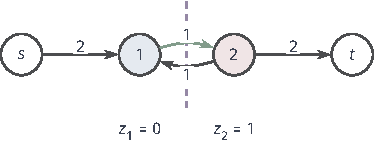
\includegraphics[width=63.281mm]{figures/01-mathematical-preliminaries-upper/07-graphs/tikz/graph-theory-binary-energy-cut/figure.pdf}
  \caption{两变量能量的割表示。点$1$在源侧、点$2$在汇侧时标签为$(0,1)$，
  两条容量$1$的反向弧中只计源侧到汇侧一条，终端弧按所在侧支付。}
  \label{fig:graph-theory-binary-energy-cut}
\end{figure}
例如$D_1=(0,2),D_2=(2,0),w_{12}=1$，四个配置能量为$2,1,5,2$，
最小割恢复$(0,1)$（图~\ref{fig:graph-theory-binary-energy-cut}）。
次模失败时$w_{i,j}<0$，不能用非负容量构造；多标签、高阶或一般非次模目标也不能自动化成一次最小割，
但特殊结构（如链）仍可能用动态规划精确求解。构造网络为$O(n+m)$，总时间还要加上所选最大流的代价。

\subsection{RatioCut谱松弛法}
\label{sec:graph-theory-ratio-cut}
以下设$n\geq2$以便分成两个非空组。单纯最小化跨组边权可能孤立一个弱连点，允许空组时零割更会直接最优。
对指示向量$\bm s=\mathbb I\{i\in S\}$，由第~\ref{chap:graph-objects}章能量式有
\begin{equation}
  \bm s^\top\bm L\bm s=\operatorname{cut}(S,\bar S),
  \label{eq:graph-theory-indicator-cut-energy}
\end{equation}
令$a=|S|>0,b=|\bar S|>0$，\term{比率割}定义为
\begin{equation}
  \operatorname{RatioCut}(S,\bar S)=\operatorname{cut}(S,\bar S)\left(\frac1a+\frac1b\right).
  \label{eq:graph-theory-ratio-cut}
\end{equation}
构造两水平向量（$S$中取$\sqrt{b/a}$、补集中取$-\sqrt{a/b}$），
\begin{equation}
  f_i=\sqrt{b/a}\ (i\in S),\qquad f_i=-\sqrt{a/b}\ (i\notin S),
  \label{eq:graph-theory-ratio-cut-balanced-vector}
\end{equation}
可直接核对$\bm1^\top\bm f=0$、$\bm f^\top\bm f=n$，且
\begin{equation}
  \bm f^\top\bm L\bm f=n\,\operatorname{RatioCut}(S,\bar S).
  \label{eq:graph-theory-ratio-cut-energy}
\end{equation}
去掉“只能取两个水平值”的限制、保留零均值与范数$n$，得到连续松弛
\begin{equation}
  \min_{\bm f^\top\bm1=0,\ \bm f^\top\bm f=n}\frac1n\bm f^\top\bm L\bm f.
  \label{eq:graph-theory-ratio-cut-relaxation}
\end{equation}
在与常量$\bm u_1=\bm1/\sqrt n$正交的子空间谱展开，Rayleigh商是$\lambda_2,\ldots,\lambda_n$的
加权平均，故不小于第二特征值$\lambda_2$，$\sqrt n\,\bm u_2$达到下界；
正权支撑连通时$\lambda_2>0$，$\bm u_2$称费德勒向量。
\begin{algorithm}[谱划分与恢复]
  建立正权支撑上的$\bm L$，求满足常量正交的第二特征方向；把坐标排序，
  在相邻不同值之间设候选阈值（相同坐标整体移动），得到两个非空组；
  逐个按原RatioCut评价，取最好的可行划分并输出其上界$U$，与有效下界$L=\lambda_2$组成证书。
\end{algorithm}
恢复时每移入一个顶点，把连向已在$S$点的边权从割中扣除、连向补集点的加上，
排序加扫描为$O(n\log n+m)$。稠密完整特征分解基准为$O(n^3)$时间、$O(n^2)$存储，
稀疏迭代的代价取决于求解器与谱间隔，不能只因$\bm L$稀疏就断言整体线性。

\subsection{NCut谱松弛法}
改用各组连接权重总量（体积）$\operatorname{vol}(S)=\sum_{i\in S}d_i^{(w)}$衡量平衡，
令$p=\operatorname{vol}(S)>0,q=\operatorname{vol}(\bar S)>0$，定义
\begin{equation}
  \operatorname{NCut}(S,\bar S)=\operatorname{cut}(S,\bar S)\left(\frac1p+\frac1q\right),
  \label{eq:graph-theory-normalized-cut}
\end{equation}
同样的两水平构造（以体积代替点数）给出$\bm y^\top\bm D\bm1=0$、
$\bm y^\top\bm D\bm y=p+q$，且$\bm y^\top\bm L\bm y=\operatorname{vol}(V)\operatorname{NCut}$。
放宽后是度加权Rayleigh问题
\begin{equation}
  \min_{\bm y\neq\bm0,\ \bm y^\top\bm D\bm1=0}
    \frac{\bm y^\top\bm L\bm y}{\bm y^\top\bm D\bm y},
  \label{eq:graph-theory-normalized-cut-relaxation}
\end{equation}
引入尺度与平衡乘子并对$\bm y$求导，左乘$\bm1^\top$用$\bm1^\top\bm L=\bm0$与平衡条件消去乘子，得
\begin{equation}
  \bm L\bm y=\lambda\bm D\bm y,\qquad \bm y^\top\bm D\bm1=0.
  \label{eq:graph-theory-normalized-cut-generalized-eigenproblem}
\end{equation}
作坐标变换$\bm x=\bm D^{1/2}\bm y$，它等价于在$\bm x\perp\bm D^{1/2}\bm1$下
求$\bm L_{\mathrm{sym}}$的第二特征向量，再变回$\bm y=\bm D^{-1/2}\bm x$；
不能把任意驻点当成最小值，也不能在一般不规则图上用组合拉普拉斯的费德勒向量替代，
只有正度正则图$\bm D=d\bm I$时方向相同、特征值缩放$1/d$。零度点体积为零要先分类处理：
若正权支撑有多个正体积分量，可直接按分量分成两个非空正体积组，得NCut为$0$。

\begin{figure}[htbp]
  \centering
  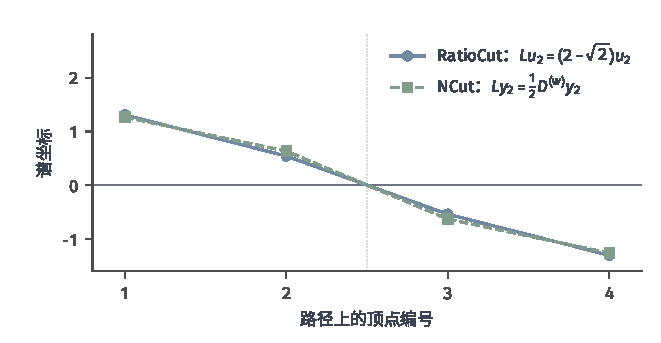
\includegraphics[width=112.0mm]{figures/01-mathematical-preliminaries-upper/07-graphs/matplotlib/graph-theory-spectral-coordinates/figure.pdf}
  \caption{单位权四点路径的两种谱方向：组合拉普拉斯第二特征向量（蓝实线）
  与度加权广义特征向量（绿虚线），二者零阈值都恢复中间分割，但相对幅度不同。}
  \label{fig:graph-theory-spectral-coordinates}
\end{figure}
在四点单位权路径$1-2-3-4$（$\bm D=\operatorname{diag}(1,2,2,1)$）上，
中间分割$\{1,2\}|\{3,4\}$的RatioCut为$1$、两水平商为$4/4=1$，
而组合$\bm L$第二特征值为$2-\sqrt2\approx0.586$、方向正比
$(1+\sqrt2,1,-1,-1-\sqrt2)$（图~\ref{fig:graph-theory-spectral-coordinates}）；
枚举七个非空二分可知离散最优RatioCut为$1$，与松弛下界并不相等。
同一分割两侧体积均为$3$，NCut为$2/3$、加权商$4/6=2/3$，广义第二特征值为$1/2$、
方向正比$(1,\tfrac12,-\tfrac12,-1)$。两法在此例恰好同分组，但方程、向量、下界均不同。
恢复后必须检查两组非空（NCut还要正体积）、重算原离散目标；
特征方向的稳定性还依赖相邻特征值间隔，重根时应考察整个子空间。

\section{本章小结}

\paragraph{按选择对象核对方法}
路径法选一条从源到目标的路线，距离变换同时处理多个位置查询，
流量法共同分配弧容量，生成树法选连接边集，匹配与指派选互不抢占的配对，
标记划分法为每个顶点选配置。同一张图、同一组数字不能省去任务定义。

\paragraph{按状态与证书理解执行}
DAG递推、Bellman--Ford和Dijkstra共享松弛动作，却分别依靠拓扑先后、
重复修正与非负边长下的永久确定；不可达$+\infty$、有限距离与负环影响的$-\infty$要分开输出。
残量增广靠撤回旧流、Kruskal靠分量防环、Prim靠跨割单边键扩树、
匹配与指派靠交替路径替换旧配对，最优性分别由流割同值、割交换或紧边势下界证书保证。

\paragraph{精确图割与谱松弛的边界}
二值次模图割在声明的有限成本条件下给出与原离散目标等价的非负容量构造；
RatioCut和NCut的特征方向只解各自的连续松弛，恢复后要检查非空或正体积、
重算原目标并用有效下界评价次优差距，两种谱方法的坐标、平衡范数与下界不能互换。
代价分析要同时计图表示、候选规模、轮数、队列或表的状态与数值精度。
下一章保持图与函数输入不变，研究顶点函数的谱坐标、滤波扩散、标记细化与配置表汇总。

\chapter{图上函数的变换与查询}
\label{chap:graph-functions}

同一张四顶点图上可以放三类很不一样的计算。给每个顶点记一个温度，得到四个可相加的实数，
任务是让相邻点的取值不要差得太悬殊；给每个顶点一个类别，得到只能比较同异的离散标记，
任务是描述它周围有哪几类邻居、各有几个；给四个二值变量一次完整赋值，
则要面对$2^4=16$种配置，任务是求总权重、最优配置或保留部分变量后的一张表。
连接结构相同，允许的运算和输出却不同，不能因为都“沿边传消息”就把它们当成一回事。

本章先在5.1节区分这三类函数对象与它们的输入输出；5.2节把顶点数值变换成由本图拉普拉斯决定的
模态坐标（图傅里叶）；5.3节按给定的频率响应处理顶点信号，包括多项式局部滤波、连续热扩散
和它的显式时间离散；5.4节处理离散标记的邻域细化；5.5节处理配置函数，
说明在什么运算规则下可以消去内部变量、怎样在树和树分解上复用接口表。
这些方法都不学习参数；具体图网络的函数族、训练与表达能力留待神经网络卷。
本章固定含$n\geq1$个顶点的有限无向非负权图，结构邻接与正权支撑沿用第~\ref{chap:graph-objects}章约定。

\section{图上函数计算的基本概念}

\paragraph{顶点数值与\term{图信号}}
给每个顶点一个实数得到$f:V\to\mathbb R$，固定顶点次序后只需存$n$个实数，称图信号。
对它做邻居加权平均会改变数值，做谱投影则改变表示而不改变信号本身——前者是处理，后者是换坐标。

\paragraph{离散顶点标记}
给每点一个类别得到$c:V\to\mathcal C$。类别首先只允许判断相同或不同，不能直接相加，
也不能未经编码把标签数字当温度求平均。要比较周围环境，需规范地保存邻居标记的种类与次数。

\paragraph{完整配置与配置函数}
给全部变量同时赋一次值得到完整配置$\bm z=(z_1,\ldots,z_n)$，
每个变量$z_i$取自非空有限集$\mathcal Z_i$，全部配置组成乘积$\prod_i\mathcal Z_i$，
四个二值变量就有$16$种。配置函数$F:\prod_i\mathcal Z_i\to\mathcal S$
给一次完整配置赋一个权重、成本或可行性结果；它评价的是整组赋值，不是某个顶点。
没有相关因子的变量仍保留自己的取值数，不能从输入里悄悄删掉。

\paragraph{输入、输出与更新时机}
对邻居温度求平均、统计邻居类别次数、对未知变量状态求和，分别输出数值、标记签名和接口表。
即使沿同一批边读取，运算对象也不同：数值处理保持顶点索引，标记细化更新类别，
配置查询则消去内部变量、保留输出变量。同步更新必须读完整旧状态、写入独立新数组，
不能边写边用本轮的新值。结构邻接供标记方法读取，实际权重供数值谱方法读取，
零权结构边可仍在但不贡献边差；图本身不自动赋予概率或因果含义。

\section{基于谱分解的图信号变换方法}
\label{sec:signal-analysis-graph-state-kernels}

规则信号的频率来自“统一平移一格”，一般图却没有对全图一致的“下一格”，
每点邻居数与方向都不同，平移算子无从定义。但“相邻取值是否接近”仍有意义，
边明确指出应比较哪些两点。因此反过来定义图频率：沿边变化小的模式为低频，变化大的为高频。
这套坐标依赖所选算子与边权，不是编号决定的，也不是先验的物理频率。

\paragraph{组合拉普拉斯的零模}
第~\ref{chap:graph-objects}章已证$\bm L\bm f=\bm0$当且仅当每条正权边两端相等；第~\ref{chap:graph-paths}章又建立了路径与连通分量。
沿正权支撑路径把这些相等关系传遍一个分量，可知同一正权支撑分量内必须取同一常数；
反之各分量独立取常数时所有正权边差为零。各分量的指示向量线性独立并张成全部这类函数，
故$\ker\bm L$由正权支撑分量的指示向量张成，零特征值重数等于这些分量的个数。
分量之间可取不同常数，零权结构边不会强制它们相同。

\paragraph{归一化零模与支撑孤点}
对$\bm L_{\mathrm{sym}}$，零能量要求每条正权边上$f_i/\sqrt{d_i}$与$f_j/\sqrt{d_j}$相等，
故每个正度分量的零空间基向量是该分量上的$\bm D^{1/2}\bm1_C$；
零度支撑孤点按零行列约定另有一个坐标零方向。普通常量零模与度缩放零模不能互换。

\paragraph{标准正交谱基与变化尺度}
有限实对称矩阵的谱定理给
\[
  \bm L=\bm U\bm\Lambda\bm U^\top,\quad \bm U^\top\bm U=\bm I,\quad
  \bm\Lambda=\operatorname{diag}(\lambda_1,\ldots,\lambda_n),\quad 0\leq\lambda_1\leq\cdots\leq\lambda_n.
\]
单位模态$\bm u_k$满足$\bm u_k^\top\bm L\bm u_k=\lambda_k$，特征值小即沿边变化小。

\subsection{实正交\term{图傅里叶变换}法}
\begin{definition}[图傅里叶变换]
  \label{def:signal-analysis-graph-fourier-transform}
  选定$\bm L$的一组实标准正交特征向量作为$\bm U$的列，图信号的图傅里叶变换及逆变换为
  \begin{equation}
    \widehat{\bm f}_{\mathcal G}=\bm U^\top\bm f,\qquad
    \bm f=\bm U\widehat{\bm f}_{\mathcal G}.
    \label{eq:signal-analysis-graph-fourier}
  \end{equation}
\end{definition}
\paragraph{投影、重构与能量}
每个坐标$\widehat f_{\mathcal G,k}=\bm u_k^\top\bm f$记录信号沿该单位模态的分量，
逆变换按$\bm f=\sum_k\widehat f_k\bm u_k$完整重构，不丢信息。并有
\[
  \|\bm f\|_2^2=\sum_k|\widehat f_k|^2,\qquad
  \bm f^\top\bm L\bm f=\sum_k\lambda_k|\widehat f_k|^2,
\]
前者是总幅值平方（不按频率加权），后者是沿边变化能量（以$\lambda_k$加权）。
在三点单位权路径上取一组标准正交基
$\bm u_0=(1,1,1)^\top/\sqrt3$、$\bm u_1=(1,0,-1)^\top/\sqrt2$、
$\bm u_2=(1,-2,1)^\top/\sqrt6$，对应特征值$0,1,3$；对$\bm f=(1,0,0)^\top$，
系数为$1/\sqrt3,1/\sqrt2,1/\sqrt6$，三个系数乘回基向量相加恰好恢复$\bm f$。

\paragraph{重特征空间与代价}
重特征值对应的子空间内可旋转正交基，单个坐标改变、子空间投影与系数平方和不变；
简单特征值的实向量也有正负号自由。跨运行比较坐标须记录基的对应，不能只比第$k$个数。
稠密完整对称特征分解通常需$O(n^3)$运算、$O(n^2)$存储，取得基后每次投影或重构为$O(n^2)$；
只求少数方向会成为截断投影，不能再称完整可逆。

\subsection{环图傅里叶变换法}
单位权简单环（$N\geq3$，每点连模$N$的左右邻居）有解析模态。其拉普拉斯逐点为
$(L f)[r]=2f[r]-f[r-1]-f[r+1]$（下标模$N$）。令$u_k[r]=N^{-1/2}e^{2\pi\mathrm i kr/N}$，代入得
\[
  L\bm u_k=\Bigl(2-2\cos\tfrac{2\pi k}{N}\Bigr)\bm u_k,
\]
有限几何和表明$\{\bm u_k\}$构成复酉基，故正变换用$\bm U^*\bm f$（共轭转置）、逆变换用$\bm U\widehat{\bm f}$。
这组复指数与信号章的DFT是同一组振荡函数：按信号章的DFT约定$X[k]=\sum_r f[r]e^{-2\pi\mathrm i kr/N}$，
图谱系数$\widehat f_k=X[k]/\sqrt N$，逆变换先乘$\sqrt N$再走含$1/N$的逆DFT。
$k$按复振荡编号而非按特征值排序，$k$与$N-k$通常是同特征值的两个相反复振荡方向，
能量不区分二者；$N=2$时左右邻居重合，不再是度$2$的上述环算子。

\paragraph{直接DFT求值与FFT求值}
直接对$N$个频率各累加$N$项需$O(N^2)$算术、$O(N)$工作数组；
同一环顺序数组也可直接调用信号章的FFT求$X$再逐项除以$\sqrt N$，
逆变换乘回$\sqrt N$后调逆FFT，长度满足分解条件时降为$O(N\log N)$，
周期边界、模式与归一化都不变。$N=4$、$\bm f=(1,0,0,0)$时四个DFT输出均为$1$、
图谱系数均为$1/2$，逆变换恢复原值，可用于两种实现的同输入核对。
一般图没有这种解析环结构，只按顶点编号调用FFT不会得到该图拉普拉斯的谱坐标。

\section{基于谱响应的图信号处理方法}

给定实标量响应$g$，在谱坐标中要求
\[
  g(\bm L)=\bm U g(\bm\Lambda)\bm U^\top,\qquad
  \bm y=g(\bm L)\bm f,\qquad \widehat y_k=g(\lambda_k)\widehat f_k.
\]
这才是信号处理——改变系数；同一特征值必须用同一响应，$g(\bm L)$才不依赖重特征空间内的任选基。
重编号$\bm L'=\bm P\bm L\bm P^\top,\bm f'=\bm P\bm f$下，标量矩阵函数天然等变：$g(\bm L')\bm f'=\bm P g(\bm L)\bm f$。

\subsection{谱分解滤波法}
已有谱基时，按“投影$\widehat{\bm f}=\bm U^\top\bm f$—逐模态缩放
$\widehat y_k=g(\lambda_k)\widehat f_k$—合成$\bm y=\bm U\widehat{\bm y}$”执行；
多列信号各列使用相同的节点算子，不把特征通道混合进图传播。
保留零模、压低高模态即为平滑；响应恒为$1$时原样恢复，丢掉部分模态则改变信号。
已有谱基时两次稠密乘法加$n$次响应求值为$O(n^2)$，首次分解另计。

\subsection{稀疏递推的多项式图滤波法}
若响应是$K$次多项式
\begin{equation}
  g(\bm L)=\sum_{r=0}^K\alpha_r\bm L^r,
  \label{eq:graph-theory-polynomial-filter}
\end{equation}
则
\begin{equation}
  \bm y=\sum_{r=0}^K\alpha_r\bm L^r\bm f,
  \label{eq:signal-analysis-polynomial-graph-filter}
\end{equation}
一次乘$\bm L$只用本点和一跳邻居，完全不必特征分解。
\begin{algorithm}[多项式图滤波]
  保存当前向量$\bm v$与累计向量$\bm y$：初始$\bm v=\bm f,\bm y=\alpha_0\bm f$；
  对$r=1,\ldots,K$，用完整旧$\bm v$算$\bm v_{\text{新}}=\bm L\bm v$写入独立缓冲，
  再令$\bm v\leftarrow\bm v_{\text{新}}$、$\bm y\leftarrow\bm y+\alpha_r\bm v$。全部顶点读完旧状态后再替换。
\end{algorithm}
按矩阵乘积的指标链，$(\bm L^r)_{ij}\neq0$要求$i,j$间存在至多$r$步的正权支撑行走，
故$K$次多项式只依赖至多$K$跳邻居；这是范围上界，范围内系数仍可能因相消为零。
由$(\bm P\bm L\bm P^\top)^r\bm P=\bm P\bm L^r$知同步稀疏递推与谱定义同样等变。
每轮稀疏乘法$O(n+m_+)$（$m_+=|E_+|$），总计$O(K(n+m_+))$，只存三个向量时额外$O(n)$。
在三点路径（特征值$0,1,3$）上取$\bm f=(1,0,0)^\top$、$H=I-L/3$（响应$1,2/3,0$），
第一轮$H\bm f=(2/3,1/3,0)^\top$（到一跳），第二轮$H^2\bm f=(5/9,1/3,1/9)^\top$（才到两跳），
与谱坐标中消去最高频模态一致。
\begin{figure}[htbp]
  \centering
  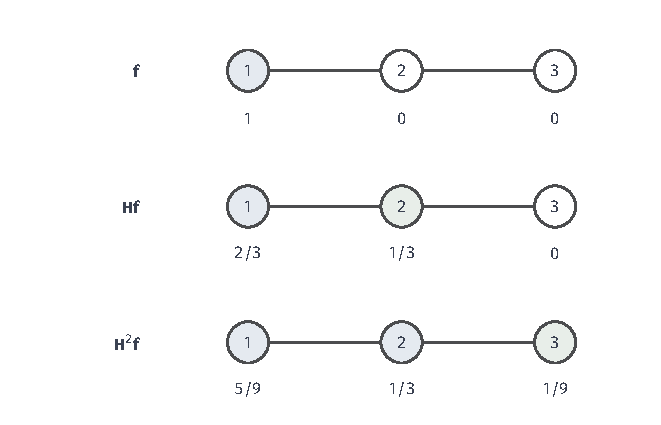
\includegraphics[width=112.0mm]{figures/01-mathematical-preliminaries-upper/05-graphs-and-signals/tikz/graph-theory-polynomial-locality/figure.pdf}
  \caption{三顶点路径上$H=I-L/3$的一次与二次作用：第一轮只到一跳邻居，
  二次多项式才到达两跳邻居。}
  \label{fig:graph-theory-polynomial-locality}
\end{figure}

\subsection{热扩散的谱求值法}
若每点按邻居与自身之差连续调整$f_i'(t)=\sum_j w_{i,j}(f_j-f_i)$，得到热方程
\begin{equation}
  \frac{\mathrm d\bm f(t)}{\mathrm dt}=-\bm L\bm f(t),\qquad \bm f(0)=\bm f_0,
  \label{eq:graph-theory-heat-equation}
\end{equation}
矩阵指数给出$\bm f(t)=e^{-t\bm L}\bm f_0
 =\sum_k e^{-t\lambda_k}\langle\bm u_k,\bm f_0\rangle\bm u_k$。
即取响应$g(\lambda)=e^{-t\lambda}$：零模保留、正模态按指数衰减。
\paragraph{总和守恒与分量均值}
由$\bm1^\top\bm L=\bm0$有$\frac{\mathrm d}{\mathrm dt}\bm1^\top\bm f=0$，总和守恒；
每个正权支撑分量分别趋于其初始平均（分量常方向投影为该分量平均），支撑连通时才是全图同一平均，
孤点保留自己的初值。贯穿图单位权、$\bm f_0=(1,0,0,0)^\top$、谱$0,2,4,4$，
保留比例为$1,e^{-2t},e^{-4t},e^{-4t}$，极限每点$1/4$而非归零（图~\ref{fig:graph-diffusion-spectrum}）。
\begin{figure}[htbp]
  \centering
  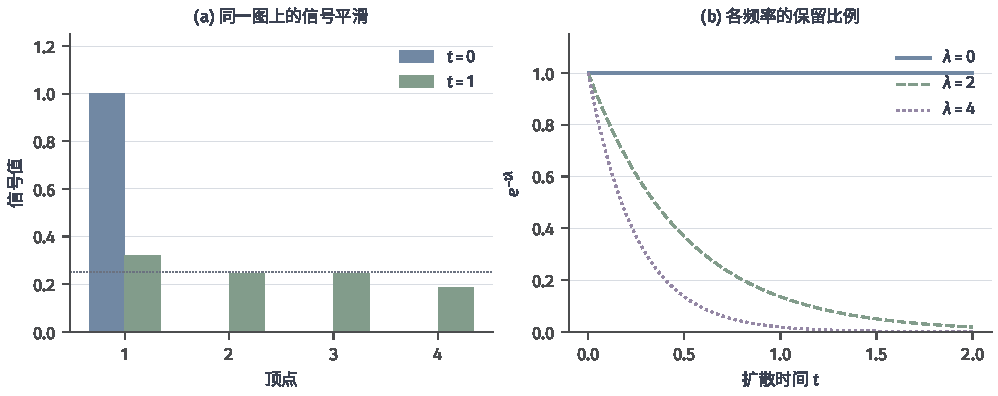
\includegraphics[width=169.0mm]{figures/01-mathematical-preliminaries-upper/05-graphs-and-signals/matplotlib/graph-diffusion-spectrum/figure.pdf}
  \caption{贯穿四顶点图的解析式扩散：左图比较初值$(1,0,0,0)$与$f(1)=e^{-L}f(0)$，
  灰线为极限均值$1/4$；右图示特征值$0,2,4$的保留比例（$4$重数为$2$）。}
  \label{fig:graph-diffusion-spectrum}
\end{figure}
\paragraph{两类耗散}
平方范数与边差能量是不同量：
\[
  \frac{\mathrm d}{\mathrm dt}\frac12\|\bm f\|_2^2=-\bm f^\top\bm L\bm f\leq0,\qquad
  \frac{\mathrm d}{\mathrm dt}(\bm f^\top\bm L\bm f)=-2\|\bm L\bm f\|_2^2\leq0.
\]
整体边差能量下降不保证每条边的差都单调缩小：三点路径从$(1,1,0)$出发，
边$1-2$初始差为零、其差的导数却为$1$，短时间内反而由相等变不等。
指数不是固定低阶多项式，不受有限$K$跳截断限制；时间过长会抹去分量内全部非恒定差异。

\subsection{显式Euler的局部扩散近似}
大图不便存完整谱基时，可用局部迭代近似固定时刻$T$的演化。
\begin{algorithm}[显式Euler扩散]
  选择整数$R\geq1$与步长$\tau=T/R$，令$\bm f^0=\bm f_0$，逐轮
  $\bm f^{r+1}=\bm f^r-\tau\bm L\bm f^r$（从旧向量算入独立新向量后整体替换），共$R$轮，输出$\bm f^R$近似$\bm f(T)$。
\end{algorithm}
按模态，$R$轮的系数乘子为$(1-\tau\lambda_k)^R$，而连续演化为$e^{-T\lambda_k}$；
固定$T$、$\tau\to0$（$R\tau=T$）时由$(1-x)$的一阶展开知这是时间离散近似，
误差还取决于输入在各模态上的系数，“迭代稳定”不等于“误差已足够小”。
若$d_{\max}=\max_i d_i>0$，取$R\geq\lceil T d_{\max}\rceil$可使$0<\tau\leq1/d_{\max}$、
每轮成为系数非负且和为$1$的邻居平均；要让$R\to\infty$（固定$\tau$、时间趋于无穷）时各非零模衰减，
需更严格的$0<\tau<1/d_{\max}$（用到$\lambda_{\max}(\bm L)\leq2d_{\max}$），
此时$|1-\tau\lambda_k|<1$，迭代趋于各分量均值。边界步长会失效：
单边两点图在$\tau=1$时每轮交换两端的值，系数虽仍非负却周期振荡、不收敛。
$R$轮共$O(R(n+m_+))$运算、额外$O(n)$，$R$由目标时长与精度决定，不能只报单轮成本。

\section{基于多重集合编码的1-WL标记细化法}

要知道每点周围有哪几类邻居、各出现几次，只记“出现过哪些类型”会丢次数，
按编号拼接又带入任意顺序；用\term{多重集合}同时保留种类与次数、忽略排列
（$\{\!\{a,a,b\}\!\}\neq\{\!\{a,b\}\!\}$）。

\begin{definition}[一维Weisfeiler--Leman细化]
  \label{def:graph-theory-wl-refinement}
  一维Weisfeiler--Leman细化（1-WL）从初始标记$c_i^{(0)}$出发，同步更新
  \begin{equation}
    c_i^{(t+1)}=\operatorname{HASH}\Bigl(
      c_i^{(t)},\ \{\!\{c_j^{(t)}:j\in N(i)\}\!\}\Bigr),
    \label{eq:graph-theory-wl-refinement}
  \end{equation}
  其中HASH对不同输入对给出不同新标记。
\end{definition}
HASH是无碰撞编码的数学约定，机器实现要比较完整键而非只比有限哈希值。
\begin{algorithm}[1-WL同步细化]
  本轮全部点只读旧标记，把自身旧标记与邻居标记多重集合组成的规范签名写入新数组，
  全部完成后统一替换；保存每轮分区与各类计数，直到某轮分区不再被拆分。
  比较两图时在两图不交并上共用初始标记规则与同一字典统一编码。
\end{algorithm}
三点路径初始同为$A$时，端点签名$(A,\{\!\{A\}\!\})$与中点签名$(A,\{\!\{A,A\}\!\})$不同，
第一轮分出端点类$B$与中心类$C$，下一轮签名再变但原有两类不再被拆开。
因新签名含自身旧标记，分区只能细分不能合并；每次严格细分至少多一个非空块，
故至多细分$n-1$次，一旦某轮未变以后也不会再分。
\begin{figure}[htbp]
  \centering
  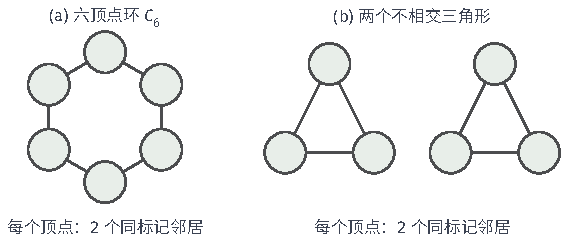
\includegraphics[width=94.936mm]{figures/01-mathematical-preliminaries-upper/05-graphs-and-signals/tikz/graph-theory-wl-local-ambiguity/figure.pdf}
  \caption{六环$C_6$与两个不相连三角形初始同标记，每点每轮都看到两个同类邻居，
  1-WL计数始终一致，无法区分连通的六环与两个分量。}
  \label{fig:graph-theory-wl-local-ambiguity}
\end{figure}
如图~\ref{fig:graph-theory-wl-local-ambiguity}，稳定不等于判同构：
六环$C_6$与两个不相连三角形的每点都看到两个同类邻居，计数始终一致，尽管连通分量数不同。
某轮两图计数不同可判定在当前属性设定下不同构，计数一直相同只表示本方法未区分；
给每点附唯一编号会改变所比较的问题（若属性随置换同步移动则是带属性图比较）。
等变只排除任意编号影响，既不保证完全可辨也不保证预测有效。
直接逐点排序邻居时一轮约需$O(n+m+\sum_i d_i\log(d_i+1))$加签名比较，轮数计入稳定前总时间。

\section{基于局部表汇总的配置查询方法}
\label{sec:graph-theory-semiring-dynamic-programming}

这类问题的一个顶点答案依赖所有其他变量，不能靠一次邻居加权汇总得到；
但局部因子只依赖少数变量，因此可以先消去内部变量、只把接口取值留在中间表。

\paragraph{总量、最优值与见证}
先看二元表$g=\begin{bmatrix}1&3\\2&4\end{bmatrix}$。解释为非负权重时，
总量$\sum_{x,y}g=10$，最大权重$\max_{x,y}g=4$（见证$(1,1)$）；
解释为成本时最小值$1$（见证$(0,0)$）。同一张表因查询不同输出不同。
保留$y$求和得$(3,7)$、再求和得$10$；只有当非负权重的总量$0<Z<\infty$时，
除以$Z$才得到概率，$Q(y)/Z$才是边缘概率，否则不能这样归一化；
最大化保留$y$得$(2,4)$，那是条件最优权重而非概率。

\paragraph{交换\term{半环}与分配规则}
一个配置内合并局部项记$\otimes$，跨未知变量的不同取值汇总记$\oplus$。
\begin{definition}[交换半环]
  \label{def:graph-theory-semiring}
  交换半环$(\mathcal S,\oplus,\otimes,e_\oplus,e_\otimes)$中两种运算都结合、交换并各有单位元，
  且$\otimes$对$\oplus$分配：
  \[
    a\otimes(b\oplus c)=(a\otimes b)\oplus(a\otimes c),\qquad a\otimes e_\oplus=e_\oplus.
  \]
  空汇总取$e_\oplus$，空组合取$e_\otimes$。
\end{definition}
半环不要求减法或除法。常用实例为：和积$(\mathbb R_{\geq0},+,\times,0,1)$、
最大积$(\mathbb R_{\geq0},\max,\times,0,1)$、最小加法
$(\mathbb R\cup\{+\infty\},\min,+,+\infty,0)$、布尔$(\{\mathrm F,\mathrm T\},\lor,\land,\mathrm F,\mathrm T)$。
最小加法约定$+\infty+c=+\infty$以表示不可行，对数最大加法则用$-\infty$。
没有相关因子的变量仍有状态数：和积下对$q$个状态汇总空组合$1$得到$q$，不能把该变量删掉。
局部因子按
\begin{equation}
  F(\bm z)=\bigotimes_a\phi_a(\bm z_{S_a})
  \label{eq:graph-theory-factorized-objective}
\end{equation}
组合，$S_a$是因子作用域；三元规则仍须整体保留为$\phi_{2,3,4}$，成对形式不是其等价分解。

\subsection{逐变量消元法}
\begin{algorithm}[变量消元]
  维护当前因子集合及按变量的反向索引。对消元序中每个$z_i$：收集全部含$i$的因子$\mathcal F_i$，
  其作用域并集去掉$i$得接口$R_i$；对每个接口配置枚举$z_i$，把旧因子投影取值后用$\otimes$组合、
  用$\oplus$累计，生成
  \[
    \psi_i(\bm z_{R_i})=\bigoplus_{z_i\in\mathcal Z_i}\bigotimes_{f\in\mathcal F_i}f;
  \]
  删除旧因子、以$\psi_i$替换并同步索引。保留变量不列入消元序；消到保留变量停止即得输出表，全消完得标量。
\end{algorithm}

\begin{theorem}[半环变量消除的正确性]
  \label{thm:graph-theory-semiring-elimination}
  对有限取值变量和交换半环，按任意完整次序消元所得标量等于直接枚举的全局汇总；
  保留一组输出变量时，消去其余变量所得表逐个配置等于原查询。
\end{theorem}
\begin{proof}
不变量是：固定剩余配置，当前因子的$\otimes$组合等于原函数对已消变量的$\oplus$汇总，
初始即原分解。消$z_i$时用分配律把不含$i$的因子移出汇总：
\[
  \bigoplus_{z_i}\Bigl[\bigotimes_{f\in\mathcal F_{-i}}f\ \otimes\bigotimes_{f\in\mathcal F_i}f\Bigr]
  =\Bigl(\bigotimes_{f\in\mathcal F_{-i}}f\Bigr)\otimes
   \Bigl(\bigoplus_{z_i}\bigotimes_{f\in\mathcal F_i}f\Bigr),
\]
末项即新因子$\psi_i$；结合、交换律把对$z_i$的汇总接到此前汇总之后，不变量保持，归纳即得结论。
\end{proof}
正确性对任意次序成立，但中间表代价由次序决定，这正是第~\ref{chap:graph-traversal}章诱导宽度$k_\pi$刻画的内容：
先消$1,4$接口只有$(z_2,z_3)$（二值$4$项），先消$2$则接口为$(z_1,z_3,z_4)$并产生填充边$1-4$（$8$项）。
第$i$步朴素代价约$O((b_i+1)q^{|R_i|+1})$，接口表与选择表各至多$q^{|R_i|}$项，
输出表还要另计$\prod_{i\in Q}|\mathcal Z_i|$个条目。
\paragraph{极值见证与混合汇总顺序}
最大/最小查询要为每个接口配置额外保存一个达到极值的$z_i$（选择表），
全消后取最后选择、再按消元逆序用已恢复接口值查表回溯；平局规则须事先声明，
最优值为$+\infty$表示无有限可行解。严格正权重可用负对数把最大积转成最小加法。
不同汇总一般不能换序：对$h=\begin{bmatrix}4&0\\0&4\end{bmatrix}$，
\begin{equation}
  \max_x\sum_y h(x,y)=4,\qquad \sum_y\max_x h(x,y)=8,
  \label{eq:graph-theory-max-sum-order-a}
\end{equation}
前者要求全部$y$共用一个$x$，后者允许$x$随$y$改变（图~\ref{fig:vol1-add-graph-max-sum-choice}）；
一般有$\max_x\sum_y h\leq\sum_y\max_x h$，等号需要存在对所有$y$同时最优的共同$x$。
\begin{figure}[htbp]
  \centering
  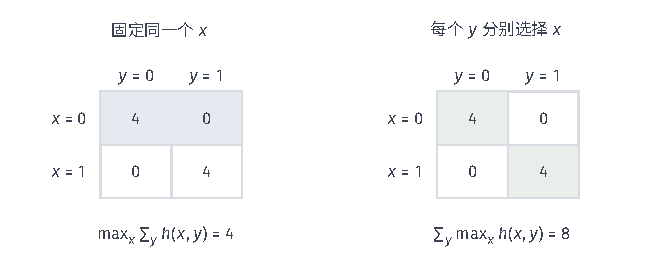
\includegraphics[width=112mm]{figures/01-mathematical-preliminaries-upper/05-graphs-and-signals/tikz/comprehension-additions/graph-max-sum-choice.pdf}
  \caption{同一表的两种汇总：左要求共用一个$x$（得$4$），右允许$x$随$y$变（得$8$）。}
  \label{fig:vol1-add-graph-max-sum-choice}
\end{figure}
混合求和与最大化会限制合法消元次序，所需宽度可能超过普通树宽；
连续积分换序还需Tonelli（非负）或Fubini（绝对可积）条件，不能只换符号。

\subsection{树上两遍消息传递法}
树的唯一路径使删边后的各侧子树互不重叠，可把子树概括成一张以接收变量为索引的消息。
\begin{theorem}[树消息递推]
  \label{thm:graph-theory-tree-message-recursion}
  对有限取值变量、有限树和交换半环，删边$\{u,v\}$后$u$侧子树$T_{u|v}$发给$v$的消息满足
  \begin{equation}
    m_{u\to v}(z_v)=\bigoplus_{z_u}\Bigl[
      \phi_u(z_u)\otimes\phi_{u,v}(z_u,z_v)
      \otimes\bigotimes_{r\in N(u)\setminus\{v\}}m_{r\to u}(z_u)\Bigr].
    \label{eq:graph-theory-tree-message-recursion}
  \end{equation}
\end{theorem}
对子树大小归纳即得：叶子无入消息、空组合取$e_\otimes$；非叶点删除$u$后各入向子树互不重叠、
彼此无边，归纳假设把它们概括为入消息，分配律把只依赖$z_u,z_v$的接口边移出各子树汇总。
每个顶点因子、内部边因子和接口边因子恰好计一次。
\begin{algorithm}[树上两遍消息]
  任选根，按后序从叶向根发消息并在根组合一元因子与全部入消息（再汇总根变量得总量，不汇总得根表）；
  需要每个变量的查询表时，再按前序向子节点发“排除该子树贡献”的向下消息
  （发给$v$时组合除$v$外各入消息，高度数点用前缀、后缀避免重复计算，半环无除法不能相除）。
\end{algorithm}
在路径$1-2-3$上取一元表$\phi_1=(1,3),\phi_2=(1,1),\phi_3=(2,1)$，边表同值为$2$、异值为$1$，
以$2$为根：$m_{1\to2}=(5,7)$、$m_{3\to2}=(5,4)$，根的一元因子最后乘入得根表$(25,28)$、总量$53$；
向下$m_{2\to1}=(14,13)$、$m_{2\to3}=(17,19)$，三个单点未归一化表分别为
$(14,39),(25,28),(34,19)$，各自求和都是$53$。和积下单点表还要除以同一正总量$53$，
最大/最小查询则沿向上消息另存选择并在定根后回溯。
$n$点树发$2(n-1)$条有向消息，每变量至多$q$状态时前后缀实现总量$O(nq^2)$、消息表共$O(nq)$项
（原始成对表可有$O(nq^2)$项）；只求一个根查询一次向上即可，不必机械回传。

\subsection{树分解下的袋消息法}
一般图先用第~\ref{chap:graph-traversal}章的有效树分解。把每个原因子整体归入唯一一个含其作用域的袋（只归一次），
本袋函数$\Phi_B$是这些因子的组合，无因子的袋取$e_\otimes$但仍保留变量域。
相邻袋$B,C$的接口$S_{B,C}=B\cap C$上，袋消息为
\[
  \mu_{B\to C}(\bm z_{S_{B,C}})
  =\bigoplus_{\bm z_{B\setminus S_{B,C}}}
   \Bigl[\Phi_B(\bm z_B)\otimes
     \bigotimes_{D\in N_{\mathcal T}(B)\setminus\{C\}}\mu_{D\to B}(\bm z_{D\cap B})\Bigr].
\]
运行交集保证删去一条袋树边后分居两侧的同一变量必在接口$S_{B,C}$中，
固定接口配置后两侧内部变量不重叠，才能沿用树归纳；同一变量在多个袋中是同一身份不是多个副本。
图~\ref{fig:graph-theory-bag-message-interface}中两袋$\{1,2,3\}$、$\{2,3,4\}$的接口$\{2,3\}$
有四个二值状态，左袋只汇总内部变量$z_1$发四行接口表，三元因子$\phi_{2,3,4}$完整归右袋，
接口因子只归一侧。若运行交集失效，同一变量在两枝被独立赋不同值，就不再对应任何全局配置。
\begin{figure}[htbp]
  \centering
  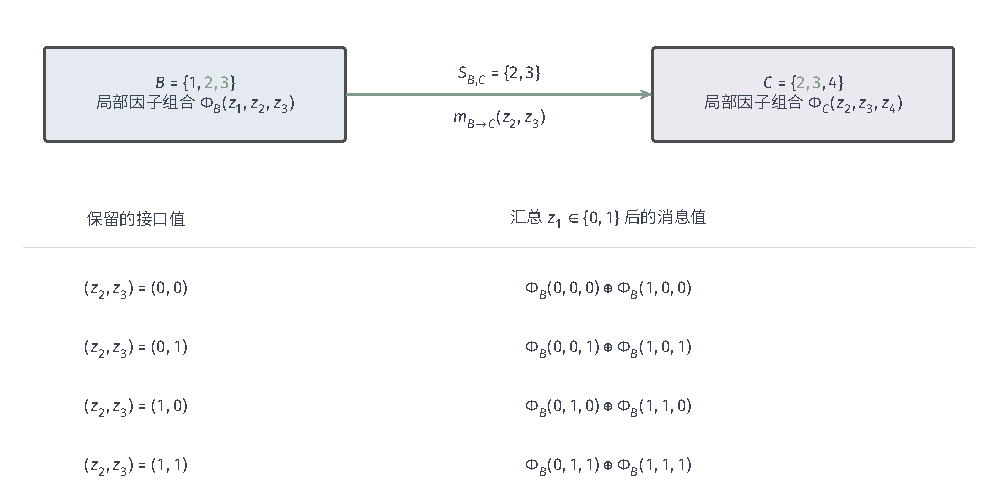
\includegraphics[width=168.998mm]{figures/01-mathematical-preliminaries-upper/05-graphs-and-signals/tikz/graph-theory-bag-message-interface/figure.pdf}
  \caption{两袋树分解上的叶袋消息：$B=\{1,2,3\}$只汇总内部变量$z_1$，
  经接口$\{2,3\}$向$C=\{2,3,4\}$发送四行二值接口表。}
  \label{fig:graph-theory-bag-message-interface}
\end{figure}
宽$k$、每变量至多$q$状态时每袋至多$q^{k+1}$个配置，一条袋消息需
$\prod_{i\in B\cap C}|\mathcal Z_i|$项，还要计袋数、因子读取、邻接袋数与每次运算成本；
固定$k,q$且袋数与表读取受多项式界时才有固定参数多项式保证，
寻找优分解本身另算。直接在原有环图上反复套树递推会因子树重叠而重复计数，
是否收敛、收敛到什么及误差都须另证，循环近似推断留待概率模型卷。

\section{本章小结}

\paragraph{坐标变换与数值处理的区别}
谱变换把顶点值写成模态坐标，完整正反变换保持信号；按响应改变系数才是滤波。
环图可借规则FFT求值，一般图的模式由所选拉普拉斯决定。有完整谱基可直接求响应，
多项式滤波用稀疏局部更新避免求全谱，热扩散给出连续演化、Euler给出需控步长与误差的离散近似；
有限跳范围与连续扩散的全图作用不能混用。

\paragraph{数值扩散与类别细化的区别}
热扩散守恒总和、保留各正权分量的初始平均，长时间抹去分量内非恒定差异，
整体能量耗散不保证逐边单调；1-WL保留邻居类型的种类与次数并只细分不合并，
但六环与双三角形不可辨，稳定不等于同构。等变只排除编号影响，不保证可辨或预测有效。

\paragraph{配置查询的运算与接口}
配置函数评价完整赋值，局部用$\otimes$组合、跨状态用$\oplus$汇总，
能否把无关因子移出汇总取决于交换半环的分配律。消元用接口表保存内部变量贡献，
树消息与袋消息在树或有效树分解上复用这些表，精确性需要有限表、合法运算、
因子唯一归属和运行交集共同保证；见证回溯、非负归一化和混合汇总顺序各有条件。
比较方法时要同时固定图表示、函数定义域、查询输出和允许运算，再计矩阵分解、
逐轮访问、表枚举、存储与回溯——小接口或局部更新不自动使所有任务便宜，输出表本身也可能很大。

回到章首三任务：温度平滑是数值处理，类别比较是标记细化，约束权重汇总是配置查询；
它们共享图这一组织，保存的数据和所得保证却各不相同。

\begin{table}[htbp]
  \centering\small
  \caption{本部分图方法的目标、关键条件与正确性依据。有限输入编码与数值误差仍须在实现中检查。}
  \label{tab:graph-algorithm-conditions}
  \begin{tabularx}{\linewidth}{@{}lX@{}}
    \toprule
    方法 & 关键条件与正确性依据\\
    \midrule
    Dijkstra最短路 & 边长非负；最小暂定点的归纳确定，输出距离与前驱\\
    Bellman--Ford & 允许负边；至多$n-1$边见证，可达负环后继标$-\infty$\\
    最小生成树 & 无向图、成本可负；割交换性质，输出最小连接树\\
    最大流最小割 & 非负容量、流守恒；可行流与同值割互相认证\\
    二部匹配/指派 & 二部、端点互斥；增广路径割证书，紧边势下界，指派$O(N^3)$\\
    树分解上配置查询 & 运行交集、有限状态、合法半环；指数依赖袋大小\\
    二值能量最小割 & 一元/成对成本有限且成对项次模；割容量与能量只差常数\\
    谱划分 & RatioCut/NCut只解连续松弛，取整回原目标并以下界评差距\\
    \bottomrule
  \end{tabularx}
\end{table}

